% This must be in the first 5 lines to tell arXiv to use pdfLaTeX, which is strongly recommended.
\pdfoutput=1
% In particular, the hyperref package requires pdfLaTeX in order to break URLs across lines.

\documentclass[11pt]{article}

% Change "review" to "final" to generate the final (sometimes called camera-ready) version.
% Change to "preprint" to generate a non-anonymous version with page numbers.
% \usepackage[review]{acl}
\usepackage[preprint]{acl}


% Standard package includes
\usepackage{times}
\usepackage{latexsym}

% For proper rendering and hyphenation of words containing Latin characters (including in bib files)
\usepackage[T1]{fontenc}
% For Vietnamese characters
% \usepackage[T5]{fontenc}
% See https://www.latex-project.org/help/documentation/encguide.pdf for other character sets

% This assumes your files are encoded as UTF8
\usepackage[utf8]{inputenc}

% This is not strictly necessary, and may be commented out,
% but it will improve the layout of the manuscript,
% and will typically save some space.
\usepackage{microtype}

% This is also not strictly necessary, and may be commented out.
% However, it will improve the aesthetics of text in
% the typewriter font.
\usepackage{inconsolata}

%Including images in your LaTeX document requires adding
%additional package(s)
\usepackage{graphicx}

% Our packages
\usepackage{booktabs}
\usepackage{subcaption}
\usepackage{multirow}
\usepackage{makecell}
\usepackage{enumitem}
\usepackage{pifont}
\usepackage{placeins}
\usepackage{stfloats}
\usepackage{amsmath}
\usepackage{amsfonts}
% \usepackage{natbib}
% % \setcitestyle{numbers,square,comma}  % 使用方括号，用逗号分隔
\usepackage{colortbl}
\usepackage{threeparttable}

\usepackage{CJKutf8}  % 使用 CJKutf8 替代 xeCJK

% 定义一个新的 prompt 展示环境
\usepackage[breakable]{tcolorbox}
\newtcolorbox{promptbox}{
    colback=gray!5,
    colframe=gray!75,
    boxrule=0.5pt,
    arc=4pt,
    left=6pt,
    right=6pt,
    top=6pt,
    bottom=6pt,
    breakable,
    fontupper=\small  % 可以使用 \small, \footnotesize, \tiny 等
}


\definecolor{lightgreen}{rgb}{0.88, 1, 0.88}
\definecolor{lightred}{rgb}{1, 0.88, 0.88}
\definecolor{lightyellow}{rgb}{1, 1, 0.88}
\definecolor{lightblue}{rgb}{0.88, 0.95, 1}
\definecolor{lightorange}{rgb}{1, 0.93, 0.88}

\newcommand{\note}[1]{\textcolor{blue}{{#1}}}
\newcommand{\task}[1]{\textcolor{red}{{#1}}}

% If the title and author information does not fit in the area allocated, uncomment the following
%
%\setlength\titlebox{<dim>}
%
% and set <dim> to something 5cm or larger.

% \title{Advancing Zero-shot Text-to-Speech Intelligibility in \\Diverse Scenarios via Preference Alignment}
% \title{Advancing Zero-shot Text-to-Speech Intelligibility \\with Preference Alignment}
% \title{Towards More Intelligible Zero-shot Text-to-Speech\\via Preference Alignment}
\title{Advancing Zero-shot Text-to-Speech Intelligibility across\\Diverse Domains via Preference Alignment}

% Author information can be set in various styles:
% For several authors from the same institution:
% \author{Author 1 \and ... \and Author n \\
%         Address line \\ ... \\ Address line}
% if the names do not fit well on one line use
%         Author 1 \\ {\bf Author 2} \\ ... \\ {\bf Author n} \\
% For authors from different institutions:
% \author{Author 1 \\ Address line \\  ... \\ Address line
%         \And  ... \And
%         Author n \\ Address line \\ ... \\ Address line}
% To start a separate ``row'' of authors use \AND, as in
% \author{Author 1 \\ Address line \\  ... \\ Address line
%         \AND
%         Author 2 \\ Address line \\ ... \\ Address line \And
%         Author 3 \\ Address line \\ ... \\ Address line}

% \author{First Author \\
%   Affiliation / Address line 1 \\
%   Affiliation / Address line 2 \\
%   Affiliation / Address line 3 \\
%   \texttt{email@domain} \\\And
%   Second Author \\
%   Affiliation / Address line 1 \\
%   Affiliation / Address line 2 \\
%   Affiliation / Address line 3 \\
%   \texttt{email@domain} \\}


\author{
\vspace{-8mm}
\\
 \textbf{Xueyao Zhang}\textsuperscript{*,1},
 \textbf{Yuancheng Wang}\textsuperscript{*,1},
 \textbf{Chaoren Wang}\textsuperscript{1},\\
 \textbf{Ziniu Li}\textsuperscript{1}, 
 \textbf{Zhuo Chen}\textsuperscript{2},
 \textbf{Zhizheng Wu}\textsuperscript{1}
\\
 \textsuperscript{1}The Chinese University of Hong Kong, Shenzhen \\
 \textsuperscript{2}ByteDance Seed
}

\begin{document}
\maketitle

\begin{abstract}
Modern zero-shot text-to-speech (TTS) systems, despite using extensive pre-training, often struggle in challenging scenarios such as tongue twisters, repeated words, code-switching, and cross-lingual synthesis, leading to intelligibility issues. To address these limitations, this paper leverages preference alignment techniques, which enable targeted construction of out-of-pretraining-distribution data to enhance performance. We introduce a new dataset, named the \underline{Int}elligibility \underline{P}reference Speech Dataset (INTP), and extend the Direct Preference Optimization (DPO) framework to accommodate diverse TTS architectures. After INTP alignment, in addition to intelligibility, we observe overall improvements including naturalness, similarity, and audio quality for multiple TTS models across diverse domains. Based on that, we also verify the weak-to-strong generalization ability of INTP for more intelligible models such as CosyVoice 2 and Ints. Moreover, we showcase the potential for further improvements through iterative alignment based on Ints. Audio samples are available at \href{https://intalign.github.io/}{https://intalign.github.io/}.
% we introduce a 3.8B \underline{In}telligibility-enhanced \underline{S}peech Language Model (Ints) and verify INTP's weak-to-strong generalization ability on this more intelligible model. Besides, we showcase the potential for further improvements through iterative alignment based on Ints. Audio samples are available at \href{https://intalign.github.io/}{https://intalign.github.io/}.
\end{abstract}

\section{Introduction}

\renewcommand{\thefootnote}{*}
\footnotetext{Equal Contribution.}

\renewcommand{\thefootnote}{\arabic{footnote}} 
\addtocounter{footnote}{0}%

% Zero-shot text-to-speech (TTS) technology has significantly advanced the field of speech synthesis. Given a target text and a reference speech as input, zero-shot TTS systems aim to synthesize the target text while mimicking the style of the reference speech, maintaining both high audio quality and speaker similarity~\cite{valle}. These techniques have a wide range of applications, including voice agents~\cite{gpt4o,doubao-voice}, virtual assistants~\cite{seedtts,cosyvoice}, and video dubbing~\cite{seedtts,maskgct}.

Despite leveraging large-scale pre-training~\cite{seedtts,maskgct,cosyvoice2}, modern zero-shot TTS systems still lack robustness during real-world applications~\cite{hallucination-survey,robustness-problem}. These systems struggle to meet even the most fundamental requirement of speech synthesis -- \textit{intelligibility}~\cite{tts-book-tanxu} in several scenarios, including: (1) the target text is hard to pronounce, such as tongue twisters or continuously repeated words~\cite{robustness-problem,seedtts}, which is referred to as \textit{articulatory} cases in this paper, (2) \textit{code-switching} cases, where the target text contains a mixture of multiple languages, and (3) \textit{cross-lingual} cases, where the languages of the target text and the reference speech differ. In these domains, existing zero-shot TTS models frequently exhibit ``hallucination'' issues, such as content insertion, omission, and mispronunciation~\cite{robustness-problem,valle}.
% \footnote{We present detailed experimental results in Section~\ref{sec:expt-main} to demonstrate the intelligibility challenge for these domains.}.


% To address these challenges, we propose to introduce \textit{preference alignment} to enhance zero-shot TTS intelligibility. Preference alignment, as a crucial post-training stage in textual large language models (LLMs), has demonstrated remarkable effectiveness in aligning model outputs with specific human values~\cite{instructgpt,RLHF-anthoropic,llama3}. The potential of this approach lies in two aspects. First, while current pre-trained TTS models lack robustness, their ``Best-of-N'' samples of multiple generations can achieve relatively high quality~\cite{maskgct}, suggesting that alignment could unlock the latent potential of these models. Second, we attribute these intelligibility challenges primarily to the sparse data distribution during pre-training -- for instance, the mismatch between training and inference in cross-lingual cases. Through preference alignment, we can create synthetic preference pairs for post-training, moving beyond the reliance on strict text-speech supervised data.

% We attribute these intelligibility challenges primarily to the problem of \textit{out-of-distribution} (OOD). For example, in cross-lingual cases, there exists a huge mismatch between monolingual pre-training and cross-lingual inference.
% % \note{modify here} 
% Previous studies indicate that by conducting multiple generations, the ``Best-of-N'' samples of pre-trained TTS models can achieve relatively high quality~\cite{maskgct,llasa}, demonstrating that these models can achieve high performance \textit{upper bounds} but suffer from \textit{instability}, thus requiring post-training elicitation to unlock their potential.

% We attribute these intelligibility challenges primarily to the problem of \textit{out-of-distribution} (OOD). For example, in cross-lingual cases, there exists a huge mismatch between monolingual pre-training and cross-lingual inference.
% Despite this instability, the models have the potential to reach high performance. Previous approaches have attempted to address this by using ``Best-of-N'' sampling~\cite{maskgct,llasa}. However, this method remains unstable and incurs high computational costs. Therefore, post-training elicitation is necessary to fully unlock the models' potential.

% To address these challenges, previous works have explored test-time based approaches, such as using ``Best-of-N'' sampling during inference~\cite{maskgct,llasa}. The effectiveness of such methods indicates that pre-trained models can achieve high performance \textit{upper bounds} but suffer from \textit{instability}.
% % , thus requiring post-training elicitation to unlock their potential. 
% We believe this instability is significantly attributed to the \textit{out-of-distribution} (OOD) problem. For example, in cross-lingual cases, there is a huge mismatch between monolingual pre-training and cross-lingual inference.

We attribute these intelligibility challenges primarily to the problem of \textit{out-of-distribution} (OOD). For example, in cross-lingual cases, there exists a huge mismatch between monolingual pre-training and cross-lingual inference. While including such scenarios in pre-training data would be a natural solution, collecting high-quality data for challenging cases like cross-lingual synthesis remains difficult. 
% Existing works propose to enhance TTS intelligibility via test-time based approaches, such as using ``Best-of-N'' sampling during inference~\cite{maskgct,llasa}. However, this method remains unstable and incurs high computational costs during inference.

Motivated by the above, we propose to use \textit{preference alignment} (PA)~\cite{instructgpt,RLHF-anthoropic} to mitigate the OOD issues, and thus enhance zero-shot TTS intelligibility. The potential of this approach lies in two aspects. 
% First, PA inherently provides a distillation effect that directly elicits the model's ``Best-of-N'' capability~\cite{iterative-dpo}. 
First, PA's \textit{customized} post-training on human expected distribution can effectively mitigate the OOD issue~\cite{zhang2024negative,li2024rl, iterative-dpo}. Second, unlike TTS pre-training that requires high-quality supervised data, PA needs only paired samples with relative preferences -- notably, even synthetic data can lead to large improvements~\cite{llama3,qwen2.5}, thus significantly simplifying data collection for challenging scenarios like cross-lingual cases. Centered on this direction, we investigate three research problems:
\vspace{-1mm}
\begin{itemize}[itemsep=0ex,leftmargin=2ex]
    \item \textbf{P1}: Dataset quality is crucial for model performance. To construct a high-quality intelligibility preference dataset, what prompts and base models should be selected, and how can we establish human-aligned preference pairs?
    \item \textbf{P2}: Unlike textual LLMs with predominantly autoregressive (AR) design, zero-shot TTS models employ diverse architectures, including AR-based~\cite{audiolm,seedtts,cosyvoice2}, Flow-Matching (FM) based~\cite{voicebox,e2tts,f5tts}, and Masked Generative Model (MGM) based~\cite{naturalspeech3,maskgct}. How can we design alignment algorithms for various architectures?
    \item \textbf{P3}: Can our preference dataset demonstrate weak-to-strong generalization~\cite{weak-to-strong-generalization}? In other words, can datasets created using less capable models effectively train more powerful models? This question is central to understanding the scalability and transferability of our dataset design.
\end{itemize}

In this paper, we address the aforementioned problems with the following key contributions:

$\rightarrow$ \textbf{P1}: We establish a synthetic \underline{Int}elligibility \underline{P}reference Speech Dataset (INTP), comprising about 250K preference pairs (over 2K hours) of diverse domains. Specifically, INTP covers multiple scenarios, utilizing various TTS models for data creation. Besides, we employ several strategies to construct preference pairs, aiming to mitigate the risk of reward hacking for simple patterns~\cite{reward-hacking,reward-hacking-wenglilian}. Particularly, we leverage human knowledge and DeepSeek-V3~\cite{deepseek-v3} to introduce perturbations into TTS systems, creating human-guided negative samples. In addition, when using Word Error Rate (WER) to determine intelligibility preferences, we not only consider self-comparison within a single model as in previous studies~\cite{tianjinchuan-pa,fpo,koel-tts}, but also introduce comparisons across different models to leverage their complementary capabilities.

$\rightarrow$ \textbf{P2}: We adopt the idea of Direct Preference Optimization (DPO)~\cite{dpo} to enhance various zero-shot TTS architectures. We employ the vanilla DPO algorithm for AR-based TTS models, while proposing extended versions of it for FM-based and MGM-based models. Our experiments on INTP shows that these algorithms effectively improve the intelligibility, naturalness, and overall quality of multiple state-of-the-art TTS systems, including ARS (AR-based)~\cite{maskgct}, F5-TTS (FM-based)~\cite{f5tts}, and MaskGCT (MGM-based)~\cite{maskgct}.

% $\rightarrow$ \textbf{P3}: To investigate the generalization ability of INTP to more powerful base models, we research the alignment of INTP for CosyVoice 2~\cite{cosyvoice2} and Ints.
% introduce an \underline{In}telligibility-enhanced \underline{S}peech Language model (Ints) to research. Specifically, we design an AR-based TTS model initialized from a textual LLM, \texttt{Phi-3.5-mini-instruct} (3.8B)~\cite{phi3}. We find that through this LLM initialization, the proposed Ints achieves remarkable performance in TTS intelligibility (Table~\ref{tab:expt-main}). Furthermore, our experimental results verify that INTP is still effective even for this more capable model, which can improve both its intelligibility and naturalness. Additionally, we showcase how to establish an \textit{iterative} preference alignment ``flywheel'' of data and model improvements~\cite{RLHF-anthoropic,llama3,iterative-dpo} based on Ints.

$\rightarrow$ \textbf{P3}: To investigate INTP's weak-to-strong generalization capability~\cite{weak-to-strong-generalization} on more powerful base models, we research its alignment effects on CosyVoice 2~\cite{cosyvoice2} and Ints (Appendix~\ref{sec:appendix-detail-ins}). Both models are initialized from textual LLMs (CosyVoice 2: from Qwen2.5, 0.5B~\cite{qwen2}. Ints: from Phi-3.5-mini-instruct, 3.8B~\cite{phi3}) and achieve superior intelligibility performance (Table~\ref{tab:expt-main}). Our experimental results verify that INTP, though constructed from weaker models, remains effective for these two strong models. Additionally, we showcase how to establish an \textit{iterative} preference alignment ``flywheel'' of data and model improvements~\cite{RLHF-anthoropic,llama3,iterative-dpo} based on Ints.

We open-source all resources used in this study at Amphion~\cite{amphion}, including: (1) the proposed INTP\footnote{\href{https://huggingface.co/datasets/amphion/INTP}{https://huggingface.co/datasets/amphion/INTP}} and DPO-based alignment codebase for various TTS models\footnote{\href{https://github.com/open-mmlab/Amphion}{https://github.com/open-mmlab/Amphion}}, (2) all the INTP-enhanced models\footnote{\href{https://huggingface.co/amphion/INTP}{https://huggingface.co/amphion/INTP}} based on Ints, CosyVoice 2, ARS, F5-TTS, and MaskGCT, and (3) our newly constructed zero-shot TTS evaluation sets across diverse domains\footnote{\href{https://huggingface.co/datasets/amphion/Amphion-TTS-Eval}{https://huggingface.co/datasets/amphion/Amphion-TTS-Eval}}.


\section{Related Work}

\paragraph{Zero-Shot Text to Speech}
Given a target text and a reference speech as input, zero-shot TTS systems aim to synthesize the target text while mimicking the reference style. Modern zero-shot TTS systems include AR approaches~\cite{valle, voicecraft, seedtts, fireredtts, cosyvoice, cosyvoice2, vevo} that model discrete speech tokens~\cite{soundstream, encodec}, and Non-AR approaches that either model continuous representations using diffusion~\cite{naturalspeech2} or flow matching~\cite{voicebox, e2tts, f5tts}, or model discrete tokens using masked generative models~\cite{soundstorm, naturalspeech3, maskgct, wang2025metis}. While these systems, trained on large-scale datasets~\cite{emilia, kahn2020libri,emilia-large}, show excellent intelligibility in regular cases~\cite{seedtts,librispeech,cosyvoice2}, they still struggle with intelligibility in real-world scenarios.

\vspace{-1mm}
\paragraph{Alignment for Speech Generation}
Alignment via post-training has demonstrated its effectiveness in the generation of text~\cite{instructgpt,RLHF-anthoropic}, vision~\cite{imagereward,tldr-perturb-vision}, speech~\cite{speechalign,seedtts,cosyvoice2}, music~\cite{musicrl}, and sound effects~\cite{tango2,baton}. In speech generation, existing works have employed preference alignment to enhance multiple aspects of speech, including intelligibility~\cite{seedtts,cosyvoice2,tianjinchuan-pa}, speaker similarity~\cite{seedtts,cosyvoice2,tianjinchuan-pa}, emotion controllability~\cite{seedtts,emo-dpo}, and overall quality~\cite{speechalign,uno,rio,dlpo,fpo,koel-tts}. 
For intelligibility, previous studies choose WER as the optimization objective, either directly employing it as a reward model~\cite{seedtts,cosyvoice2} or centering around it to construct preference pairs~\cite{tianjinchuan-pa,fpo,koel-tts}. 

However, the existing research exhibits two main limitations. First, in constructing intelligibility preference dataset, current works rely solely on a single model to generate data~\cite{tianjinchuan-pa,fpo,koel-tts}, neglecting comparisons across different models. Additionally, beyond the objective WER, the potential of leveraging human knowledge or feedback to construct preference pairs remains unexplored. Second, most existing work has focused primarily on optimizing AR-based~\cite{speechalign,seedtts,cosyvoice2,tianjinchuan-pa} or diffusion-based~\cite{dlpo} TTS models, leaving open the question of how to design effective alignment algorithms for other architectural paradigms, such as FM-based and MGM-based TTS models.


\section{INTP: Intelligibility Preference Speech Dataset}

\begin{table*}[t]
\begin{center}
\begin{threeparttable}
    \begin{minipage}{0.68\textwidth}
    \subfloat[Distribution of preference pairs, where pronunciation-perturbed and punctuation-perturbed texts are introduced to create the human-guided negative samples.\label{tab:intp-stats}]{
    \resizebox{\textwidth}{!}{
    \begin{tabular}{r|ccccc|c}
        \toprule
         & \textbf{\makecell[c]{Regular}} & \textbf{\makecell[c]{Repeated}} & \textbf{\makecell[c]{Code-Switching}} & \textbf{\makecell[c]{Pronunciation-\\perturbed}} & \textbf{\makecell[c]{Punctuation-\\perturbed}} & \textbf{\#Total} \\
        \midrule
        \textbf{ARS}~\cite{maskgct} & 8,219 & 8,852 & 8,300 & 7,325 & 8,036 & 40,732 \\
        \textbf{F5-TTS}~\cite{f5tts} & 8,425 & 8,555 & 7,976 & 7,909 & 6,667 & 39,532 \\
        \textbf{MaskGCT}~\cite{maskgct} & 9,055 & 10,263 & 8,289 & 7,604 & 7,686 & 42,897 \\
        \midrule
        \textbf{Intra Pairs} & 25,699 & 27,670 & 24,565 & 22,838 & 22,389 & 123,161 \\
        \textbf{Inter Pairs} & 27,008 & 27,676 & 24,651 & 25,045 & 23,970 & 128,350 \\
        \midrule
        \textbf{\#Total} & 52,707 & 55,346 & 49,216 & 47,883 & 46,359 & 251,511 \\
        \bottomrule
    \end{tabular}
    }
    }
    \end{minipage}%
    \hfill
    \begin{minipage}{0.3\textwidth}
    \subfloat[Examples of different types for a text, ``\textit{A panda eats shoots and leaves}''.\label{tab:intp-examples}]{
    \resizebox{\textwidth}{!}{
    \begin{tabular}{r|l}
    \toprule
     \textbf{Text Type} & \textbf{Example} \\
     \midrule
     \textbf{Regular} & \textit{A panda eats shoots and leaves.} \\ \cmidrule(lr){1-2}
     \textbf{Repeated} & \textit{\makecell[l]{A panda panda eats shoots and\\leaves and leaves and leaves.}} \\ \cmidrule(lr){1-2}
     \textbf{Code-Switching} & 
        \begin{CJK*}{UTF8}{gbsn}
            \textit{熊猫吃~shoots~和~leaves。}
        \end{CJK*} \\ \cmidrule(lr){1-2}
    \textbf{\makecell[r]{Pronunciation-\\perturbed}} & \textit{A pan duh eights shots n leafs.} \\ \cmidrule(lr){1-2}
    \textbf{\makecell[r]{Punctuation-\\perturbed}} & \textit{A panda eats, shoots, and leaves.} \\
    \bottomrule
    \end{tabular}
    }
    }
    \end{minipage}
    \vspace{-2mm}
\end{threeparttable}
\caption{Intelligibility Preference dataset (INTP). There are about 250K pairs (over 2K hours) in INTP, covering various texts and speechs, multiple models, and diverse preference pairs.}
\label{tab:intp}
\vspace{-3mm}
\end{center}
\end{table*}

% Statistics of the proposed Intelligibility Preference Dataset (INTP). There are about 250K pairs (over 2K hours) in INTP, covering various text types, where pronunciation-perturbed and punctuation-perturbed texts are introduced in this study to create the human-guided negative samples (Section 3.3).

To enhance the TTS intelligibility, this study opts for constructing a preference dataset to align~\cite{tianjinchuan-pa,fpo,koel-tts} rather than directly optimizing single metrics or rules such as WER~\cite{seedtts,cosyvoice2}. This choice is motivated by two key considerations. First, through the construction of a preference dataset, we can inject human knowledge and feedback beyond WER, such as creating human-guided negative samples in the framework of preference alignment (Section~\ref{sec:human-guided-negative}). Second, in addition to the existing approach of constructing preference pairs from multiple samples of a single model~\cite{tianjinchuan-pa,fpo,koel-tts}, we can leverage comparisons across different models to create preference pairs, thereby utilizing the complementary capabilities of various models (Figure~\ref{fig:inter-pair}). These different strategies help increase diversity in the dataset, mitigating the risk of ``reward hacking'' that often results from the simple patterns inherent in single metrics or rules~\cite{RLHF-anthoropic,reward-hacking,reward-hacking-wenglilian}.

% Existing approaches to intelligibility preference alignment can be categorized into two main approaches. The first directly employs WER either as a reward model~\cite{seedtts} or introduces it as a differentiated loss~\cite{cosyvoice2} for optimization. The second utilizes WER as an objective metric to construct preference pairs, which are then used to train an (explicit~\cite{reinforce,ppo} or implicit~\citep{dpo}) reward model. For instance, we can sample a model multiple times for the same prompt, where samples with lower WER scores are treated as positive samples, while those with higher WER scores are considered negative samples~\cite{cosyvoice2,tianjinchuan-pa,fpo}.

Formally, we aim to construct an intelligibility preference dataset $\mathcal{D} = \{(x, y^w, y^l)\}$, where each triplet comprises a prompt $x$ (consisting of target text $x^{text}$ and reference speech $x^{speech}$ for zero-shot TTS models), along with a pair of synthesized speech samples $(y^w, y^l)$. Here, $y^w$ and $y^l$ represent the preferred (positive) and dispreferred (negative) outputs conditioned on $x$, respectively. Statistics of the proposed INTP are presented in Table~\ref{tab:intp}. 
% In the following sections, we first detail the construction process of INTP (Section~\ref{sec:prompt-construction}-\ref{sec:preference-pairs-construction}), followed by an analysis of how well the constructed INTP aligns with human values (Section~\ref{sec:intp-human-verify}).

\subsection{Prompt Construction}\label{sec:prompt-construction}

To establish a high-quality preference dataset, we aim to make the distribution of prompt $x$ cover a wide range of domains. For the target text $x^{text}$, from the linguistic perspective, we design three distinct categories: (1) \textbf{Regular text}, which represents the general cases for TTS systems, aimed at enhancing model intelligibility in common scenarios; (2) \textbf{Repeated text}, which contains repeated or redundant words and phrases, specifically designed to improve TTS performance in articulatory cases; and (3) \textbf{Code-switching text}, which incorporates a mixture of different languages, intended to enhance TTS capabilities in multilingual scenarios. From the semantic perspective, we collect text content across diverse topics and domains to enrich the distribution of $x^{text}$. For the reference speech $x^{speech}$, we aim to cover a wide range of speakers, speaking styles, and acoustic environments. Regarding the pairing of $x^{text}$ and $x^{speech}$, we further consider their language alignment by constructing both \textbf{monolingual} and \textbf{cross-lingual} combinations (more statistics in Appendix~\ref{sec:appendix-prompt-construction}).

We construct these prompt data based on the Emilia-Large~\cite{emilia,emilia-large}, which contains real-world speech data and textual transcriptions across diverse topics, scenarios, and speaker styles. We perform stratified sampling on Emilia-Large's speech and text data to obtain multilingual prompts. We employ DeepSeek-V3~\cite{deepseek-v3} to preprocess the sampled text, including typo correction, and use it as regular text. Based on these regular texts, we further utilize DeepSeek-V3 to transform them into different text types (as shown in Table~\ref{tab:intp-examples}). Construction details are provided in Appendix~\ref{sec:appendix-prompt-construction}.

% \vspace{-2mm}
\subsection{Model Selection}

\begin{figure}[t]
    \centering
    \begin{subfigure}[b]{0.49\columnwidth}
        \centering
        
\includegraphics[width=\textwidth]{img/pair-intra.png}
        \caption{Intra Pair}
        \label{fig:intra-pair}
    \end{subfigure}
    \hfill
    \begin{subfigure}[b]{0.49\columnwidth}
        \centering
        
\includegraphics[width=\textwidth]{img/pair-inter.png}
        \caption{Inter Pair}
        \label{fig:inter-pair}
    \end{subfigure}
    \hfill
    \begin{subfigure}[b]{0.49\columnwidth}
        \centering
        
\includegraphics[width=\textwidth]{img/pair-perturbed.png}
        \caption{Perturbed Pair}
        \label{fig:perturbed-pair}
        \vspace{-3mm}
    \end{subfigure}
    \caption{Three kinds of preference pairs in INTP.}
    \label{fig:preference-pairs}
    \vspace{-5mm}
\end{figure}

We utilize multiple zero-shot TTS models with diverse architectures for data synthesis to enhance INTP's diversity and generalization. Specifically, we select the following three models:
(1) \textbf{ARS} (AR-based): Introduced as an autoregressive baseline by~\citet{maskgct}. and referred to as ``AR + SoundStorm'' in the original paper~\cite{maskgct}. It adopts a cascaded architecture, including the autoregressive \textit{text-to-codec} and the non-autoregressive \textit{codec-to-waveform}~\cite{soundstorm}.
(2) \textbf{F5-TTS} (FM-based): It follows E2 TTS~\cite{e2tts} and uses a flow-matching transformer~\cite{voicebox,flow-matching} to convert the text to acoustic features directly~\cite{f5tts}.
(3) \textbf{MaskGCT} (MGM-based): Similar to ARS, MaskGCT employs a two-stage architecture. The key distinction lies in its use of an MGM in the text-to-codec stage~\cite{maskgct}.

All the three are pre-trained on Emilia~\cite{emilia} (about 100K hours of multilingual data) and represent state-of-the-art zero-shot TTS systems across different architectures. We utilize their officially released pre-trained models (see Appendix~\ref{sec:appendix-model-selection} for details) to generate data for INTP.

\subsection{Preference Pairs Construction}\label{sec:preference-pairs-construction}

In constructing intelligibility preference pairs, we design three categories of pairs (Figure~\ref{fig:preference-pairs}):

\paragraph{Intra Pair} 
These pairs are generated through model self-comparison (Figure~\ref{fig:intra-pair}), following an approach similar to previous studies~\cite{tianjinchuan-pa,fpo,koel-tts}. For a given prompt $x$, we conduct multiple samplings using the same model. Subsequently, we calculate the WER for each generation and designate the samples with the lowest and highest WER as $y^w$ and $y^l$, respectively. To enlarge the gap between $y^w$ and $y^l$, we employ diverse sampling hyperparameters across multiple generations from the same model. Additionally, we use a specific WER threshold to filter out pairs with insufficient performance gaps (more details in Appendix~\ref{sec:appendix-intp-intra-pair}).

\paragraph{Inter Pair} 
These pairs are constructed by comparing outputs across different models (Figure~\ref{fig:inter-pair}). The efficacy of this approach lies in leveraging the complementary strengths of various models. For example, by comparing intra-pairs from different models for the same prompt, we can identify the ``best of the best'' samples, thereby enhancing the overall quality of positive samples in our dataset. Similar to intra pair, we also employ WER to identify intelligibility preferences for inter pairs (see Appendix~\ref{sec:appendix-intp-inter-pair} for details).

Notably, the proposed inter-pair construction pipeline enables comparative evaluation of intelligibility performance across different models. Using this pipeline, we compared four state-of-the-art models in the field: ARS~\cite{maskgct}, F5-TTS~\cite{f5tts}, MaskGCT~\cite{maskgct}, and CosyVoice 2~\cite{cosyvoice2}. We constructed 10K inter-pairs and analyzed the win rates of these models, as shown in Table~\ref{tab:intp-inter-arena}. Interestingly, even ARS, the model with the lowest win rate, achieves a 4.1\% success rate against the strongest model, CosyVoice 2. This finding validates our assumption regarding the complementary capabilities among various models.

\paragraph{Perturbed Pair}\label{sec:human-guided-negative}
In addition to the aforementioned two types of pairs which are established based on WER, we leverage human knowledge and DeepSeek-V3~\cite{deepseek-v3} to create human-guided negative samples, termed perturbed pairs (Figure~\ref{fig:perturbed-pair}). The main idea involves deliberately perturbing the input prompt, thereby inducing the model to generate low-quality samples~\cite{tango2,tldr-perturb-vision}. 
% By providing these negative samples, we guide the model's exploration in the preference learning process by eliminating such unfavorable regions of the search space.

We design two types of perturbation for the target text in the prompt (as shown in Table~\ref{tab:intp-examples}): (1) \textbf{Pronunciation perturbation}: we replace certain characters of the text with easily mispronounceable alternatives. For example, given the text ``\textit{A panda eats shoots and leaves}'', we can create the perturbed text ``\textit{A pan duh eights shots n leafs}''. (2) \textbf{Punctuation perturbation}: we modify the punctuation, such as commas, to alter pause patterns and prosody in the text. For example, by adding commas to the text ``\textit{A panda eats shoots and leaves}'', we obtain ``\textit{A panda eats, shoots, and leaves}'', where the words ``\textit{shoots}'' and ``\textit{leaves}'' transform from nouns in the original text to verbs, creating a significant semantic shift. The detailed construction process is provided in Appendix~\ref{sec:appendix-intp-perturbed-pair}.


\subsection{Human Perception Verification}\label{sec:intp-human-verify}

\begin{table}[t]
\begin{center}
\resizebox{\columnwidth}{!}{%
\begin{threeparttable}
    \begin{tabular}{c|cccc|c}
        \toprule
         & \textbf{ARS} & \textbf{F5-TTS} & \textbf{MaskGCT} & \textbf{CosyVoice 2} & \textbf{Win Rate} ($\uparrow$) \\
        \midrule
        \textbf{ARS} & / & 6.7\% & 7.4\% & 4.1\% & 18.3\% \\
        \textbf{F5-TTS} & 10.4\% & / & 8.8\% & 5.9\% & 25.1\% \\
        \textbf{MaskGCT} & 10.4\% & 8.0\% & / & 5.9\% & 24.3\% \\
        \textbf{CosyVoice 2} & 11.9\% & 10.2\% & 10.3\% & / & 32.3\% \\
        \bottomrule
    \end{tabular}
    \begin{tablenotes}
        {
        \item[*] The percentage in each cell represents the proportion of cases where the model on the horizontal axis outperforms the model on the vertical axis. 
        \item[*] The \textbf{Win Rate} is calculated as the sum of values from columns 2 through 5.
        }
    \end{tablenotes}
\end{threeparttable}
}
\caption{TTS Intelligibility Arena: We employ the inter-pair construction from INTP to compare intelligibility among four state-of-the-art zero-shot TTS models.}
\label{tab:intp-inter-arena}
\vspace{-4mm}
\end{center}
\end{table}

\begin{table}[t]
\begin{center}
\resizebox{\columnwidth}{!}{%
\begin{threeparttable}
    \begin{tabular}{c|cccc}
        \toprule
         & \makecell[c]{\textbf{ARS}} & \makecell[c]{\textbf{F5-TTS}} & \makecell[c]{\textbf{MaskGCT}} & \makecell[c]{\textbf{CosyVoice 2}} \\
         \midrule
         \textbf{Positive Samples} & 73.0\% & 88.1\% & 90.9\% & 100.0\% \\
         \textbf{Negative Samples} & 45.7\% & 15.8\% & 47.1\% & 75.0\% \\
         \midrule
         \textbf{All} & 59.7\% & 53.7\% & 64.3\% & 90.4\% \\
         \bottomrule
    \end{tabular}
    % \begin{tablenotes}
    %     \item[*] We use the intra-pair pipeline of INTP to generate the postive/negative samples.
    % \end{tablenotes}
    % \vspace{-3mm}
\end{threeparttable}
}
\caption{Human-annotated reading accuracy ($\uparrow$) for four state-of-the-art zero-shot TTS models on regular texts. We use the intra-pair pipeline of INTP to generate the positive and negative samples.}
\label{tab:human-read-acc-verify}
\vspace{-5mm}
\end{center}
\end{table}

After constructing INTP, we further conducted subjective evaluation to verify its alignment with human perception. For intelligibility alignment, we design a \textbf{reading accuracy} listening task (see Appendix~\ref{sec:appendix-sub-eval} for details): given a text and a speech, subjects perform binary classification to determine whether the speech accurately reads the text without any content insertion, omission, or mispronunciation. Using four state-of-the-art zero-shot TTS models, we generate 300 intra-pairs on INTP regular texts. The results in Table~\ref{tab:human-read-acc-verify} demonstrate that INTP's preference identification for intra pairs aligns well with human judgments of intelligibility. Furthermore, comparing Tables~\ref{tab:intp-inter-arena} and \ref{tab:human-read-acc-verify} reveals that INTP's inter-pair comparisons of intelligibility across different models also effectively align with human values.

In addition to intelligibility, we also investigated how well INTP aligns with human preferences for \textit{naturalness}, which is one of the most general-purpose metrics for TTS~\cite{tts-book-tanxu}. The experimental results demonstrate that the naturalness gap between positive and negative samples of INTP is substantial and perceptible to human listeners. We discuss this finding in details in Appendix~\ref{sec:appendix-intp-human-verficiation}.


\section{Preference Alignment for Diverse Zero-Shot TTS models}\label{method:dpo}

In this section, we present methods for achieving preference alignment across a range of TTS models, including autoregressive based, flow-matching based, and masked generative model based architectures. Building on the framework of Direct Preference Optimization (DPO)~\cite{dpo}, initially developed for AR-based models, we adapt and extend its principles to FM-based and MGM-based models. We note that DPO is computationally efficient in practice, and its iterative variant aligns seamlessly with the online reinforcement learning (RL) framework \citep{li2023rema4}.

% In this section, we present methods for preference alignment across various TTS models, including AR-based, FM-based, and MGM-based. We will adopt and extend the framework of Direct Preference Optimization (DPO)~\cite{dpo}, originally designed for AR-based models to FM-based and MGM-based.

% Particulalry, we adopt the unified optimization idea, Direct Preference Optimization (DPO)~\cite{dpo}, across different models. 
% We start by introducing DPO for AR models, its original design paradigm. Then, we detail how to extend DPO to flow-matching and masked generative models.

\subsection{DPO for AR Models}
\label{method:dpo_ar}

% Performance alignment in our work aims to optimize TTS models for improved intelligibility in diverse domains. 
The main idea of reinforcement learning (RL) for preference alignment is to introduce a reward model  $r(x,y)$ to guide the model for improvement (see e.g., \citep{li2023rema4}). Here $y$ represents the output (i.e., the generated speech in zero-shot TTS), and $x$ means the input prompt (i.e., the reference speech and the target text in zero-shot TTS).
% A common approach to achieving preference alignment is reinforcement learning (RL), where a latent reward model $r(x, y)$ is introduced to quantify $y$ given $x$.
% \textit{In the context of zero-shot TTS, $y$ represents the generated speech, while $x$ comprises the text and the prompt speech.}
% There are multiple approaches to modeling preferences for training $r(x, y)$,
A widely adopted reward model design is based on Bradley-Terry (BT) model, which defines the probability of preferred sample $y^w$ over dispreferred sample $y^l$ given $x$ as $p_\text{BT}(y^w \succ y^l \mid x) = \sigma (r(x, y^w) - r(x, y^l))$.
We can train the reward model \( r_\phi(x, y) \) by minimizing the negative log-likelihood of observed comparisons from the preference dataset $\mathcal{D}$:
% \vspace{-2mm}
\begin{equation}
    {\small
    \begin{aligned}
 \mathcal{L}_\text{R} = -\mathbb{E}_{(x, y_w, y_l) \sim \mathcal{D}} \left[ \log \sigma\left(r_\phi(x, y_w) - r_\phi(x, y_l)\right) \right].
    \end{aligned}
    }
\label{eq:reward_model}
\end{equation}
With the given reward model, the RL optimization objective is to guide the model to maximize the expected reward while minimizing the KL-divergence from a reference distribution:
% \vspace{-2mm}
\begin{equation}
    {\small
    \begin{aligned}
  \max_{p_\theta} \mathbb{E}_{x, y \sim p_\theta(y | x)} [r(x, y)] - \beta D_{\text{KL}} [p_\theta(y | x) \parallel p_{\text{ref}}(y | x)],  
  \end{aligned}
  }
\label{eq:rl_obj}
\end{equation}
where the hyperparameter $\beta$ controls the strength of the regularization.
As highlighted in~\citet{dpo}, the optimization problem in Equation~\ref{eq:rl_obj} admits a closed form solution. This implies a direct relationship between the reward function and the policy. Substituting the reward expression into Equation~\ref{eq:reward_model} leads the DPO loss:
\begin{equation}
    {\small
    \begin{aligned}
\mathcal{L}_\text{DPO} = -\mathbb{E}_{\mathcal{D}} \left[ \log \sigma\left( \beta \left( \log \tfrac{p_\theta(y_w | x)}{p_{\text{ref}}(y_w | x)} - \log \tfrac{p_\theta(y_l | x)}{p_{\text{ref}}(y_l | x)} \right) \right) \right].
    \end{aligned}
    }
\label{eq:dpo_ar}
\end{equation}

% As highlighted in~\citet{dpo}, the optimization problem in Equation~\ref{eq:rl_obj} admits a closed form solution. Specifically, the optimal policy \( p_\theta^*(y | x) \) that maximizes the RL objective can be expressed as:
% \begin{equation}
%     {\small
%     \begin{aligned}
% p_\theta^*(y | x) = \frac{1}{Z(x)} p_{\text{ref}}(y | x) \exp\left(\frac{1}{\beta} r(x, y)\right),
%     \end{aligned}
%     }
% \label{eq:optimal_policy}
% \end{equation}
% where \( Z(x) \) is the partition function ensuring normalization. Crucially, this implies a direct relationship between the reward function and the policy:  
% \begin{equation}
%     {\small
%     \begin{aligned}
%     r(x, y) = \beta \log \frac{p_\theta^*(y | x)}{p_{\text{ref}}(y | x)} + \beta \log Z(x).
%     \end{aligned}
%     }
% \label{eq:reward_expression}
% \end{equation}
% Substituting this reward expression (Equation~\ref{eq:reward_expression}) into the loss function of reward modeling (Equation~\ref{eq:reward_model}) leads the DPO loss:
% \begin{equation}
%     {\small
%     \begin{aligned}
% \mathcal{L}_\text{DPO} = -\mathbb{E}_{\mathcal{D}} \left[ \log \sigma\left( \beta \left( \log \tfrac{p_\theta(y_w | x)}{p_{\text{ref}}(y_w | x)} - \log \tfrac{p_\theta(y_l | x)}{p_{\text{ref}}(y_l | x)} \right) \right) \right].
%     \end{aligned}
%     }
% \end{equation}


DPO enables direct preference alignment for AR-based TTS models, eliminating the need for explicit reward modeling or RL optimization. In the following subsections, we will introduce its extensions for FM-based and MGM-based TTS models.

\subsection{DPO for Flow-Matching Models}
\label{method:dpo_fm}

The vanilla DPO algorithm is tailored for AR models, while~\citet{wallace2024diffusion} extends it to diffusion models. In this subsection, we introduce the DPO algorithm for flow-matching models, specifically demonstrating its application to optimal transport flow-matching (OT-FM), a common approach in FM-based TTS models~\cite{voicebox,e2tts,f5tts}.
Given the continuous representation $y$ of a speech sample and its corresponding condition $x$, OT-FM constructs a linear interpolation path between Gaussian noise $y_0 \sim \mathcal{N}(0, I)$ and the target data $y_1 = y$. Specifically, the interpolation follows $y_t = (1-t)y_0 + t\,y_1$, where $t \in [0,1]$,
which naturally induces a velocity field \( v_\theta(y_t, t, x) \) that captures the constant directional derivative
$\frac{dy_t}{dt} = y_1 - y_0$.
OT-FM aims to learn the velocity field to match the true derivative. The corresponding loss function is defined as
% \vspace{-2mm}
\begin{equation}
{\small
\begin{aligned}
\mathcal{L}_{\text{OT-FM}} = \mathbb{E}_{y_0, y_1, x, t}
\|\,v_\theta(y_t,t,x) - \left(y_1 - y_0\right)\|_2^2,
\end{aligned}
}
\label{eq:obj_fm}
\end{equation}
where $t$ is the time step that is sampled from the uniform distribution $\mathcal{U}(0, 1)$.

% Now, we present DPO for flow matching. 
Inspired by~\citet{wallace2024diffusion}, we rewrite the RL objective for flow-matching models. Let $p_\theta(y_1|y_t,t,x)$ denote our policy that predicts the target sample $y_1$ given the noised observation $y_t$ at time $t$ and condition $x$. We initialize from a reference flow-matching policy $p_{\text{ref}}$. The RL objective can be written as:
% \vspace{-2mm}
\begin{equation}
{\small
\begin{aligned}
\max_{p_\theta} & \mathbb{E}_{y_1 \sim p_\theta(y_1|x), t, x}[r(y_1,x)] \\
& - \beta \mathbb{D}_{\text{KL}}[p_\theta(y_1|y_t,t,x) \| p_{\text{ref}}(y_1|y_t,t,x)].
\end{aligned}
}
\label{eq:rl_obj_fm}
\end{equation}
Following a similar derivation process as in DPO (we provide more details in Appendix~\ref{sec:appendix-derivation-fm}), we can obtain the loss function for flow-matching DPO:
% \vspace{-2mm}
\begin{equation}
{\scriptsize
\begin{aligned}
& \mathcal{L}_{\text{DPO-FM}} = -
\mathbb{E}_{(y_1^w, y_1^l, x) \sim \mathcal{D}, t} \\
& \log \sigma \left( \beta \left( \log \frac{p_\theta(y_1^w|y_t^w,t,x)}{p_{\text{ref}}(y_1^w|y_t^w,t,x)}
- \log \frac{p_\theta(y_1^l|y_t^l,t,x)}{p_{\text{ref}}(y_1^l|y_t^l,t,x)} \right) \right),
\end{aligned}
}
\label{eq:dpo-fm}
\end{equation}
% where $y_1^w$ and $y_1^l$ represent the ``winning'' and ``losing'' samples from the preference dataset, while $y_t^w$ and $y_t^l$ are the interpolations at time $t$ between $y_1^w$ and $y_1^l$ and the randomly sampled $y_0^w$ and $y_0^l$. The loss can be transformed into the velocity space:
where $y_1^w$ and $y_1^l$ represent the preferred and dispreferred samples from the preference dataset, respectively, while $y_t^w$ and $y_t^l$ are the interpolations at time $t$ between $y_1^w$ and $y_1^l$ and the randomly sampled $y_0^w$ and $y_0^l$. The loss can be transformed into the velocity space:
\vspace{-2mm}
\begin{equation}
{\tiny
\begin{split}
& \mathcal{L}_{\text{DPO-FM}} = -\mathbb{E}_{(y_1^w, y_1^l, x) \sim \mathcal{D}, t} \log \sigma \Big( -\beta \\
& \Big( \left\| v_\theta(y^w_t, t, x) - (y_1^w - y_0^w) \right\|_2^2
- \left\| v_\text{ref}(y^w_t, t, x) - (y_1^w - y_0^w) \right\|_2^2 \Big) \\
& - \Big( \left\| v_\theta(y^l_t, t, x) - (y_1^l - y_0^l) \right\|_2^2
- \left\| v_\text{ref}(y^l_t, t, x) - (y_1^l -y_0^l) \right\|_2^2 \Big) \Big).
\end{split}
}
\label{eq:dpo-fm-velocity}
\end{equation}

This proposed algorithm can be applied to a wide range of FM-based and diffusion-based TTS models~\cite{voicebox, e2tts, naturalspeech2}. In this study, we use it to optimize F5-TTS~\cite{f5tts} as a representative.

\begin{table*}[t]
\begin{center}
\begin{threeparttable}
    \resizebox{\textwidth}{!}{
    \begin{tabular}{l||rrc|rrc|rrc|rrc||rrc}
    \toprule
    \multirow{2}{*}{\textbf{Model}} & 
    \multicolumn{3}{c|}{\textbf{Regular cases}} &
    \multicolumn{3}{c|}{\textbf{Articulatory cases}} &
    \multicolumn{3}{c|}{\textbf{Code-switching cases}} &
    \multicolumn{3}{c||}{\textbf{Cross-lingual cases}} &
    \multicolumn{3}{c}{\textbf{Avg}} \\
    \cmidrule(lr){2-13} \cmidrule(lr){14-16}
     & \textbf{WER} & \textbf{SIM} & \textbf{N-CMOS} & \textbf{WER} & \textbf{SIM} & \textbf{N-CMOS} & \textbf{WER} & \textbf{SIM} & \textbf{N-CMOS} & \textbf{WER} & \textbf{SIM} & \textbf{N-CMOS} & \textbf{WER} & \textbf{SIM} & \textbf{N-CMOS} \\
    \midrule
    % ----- ARS -----
    \multicolumn{1}{l||}{\textbf{ARS}}
        & 3.96 & 0.717 & -
        & 20.03 & 0.693 & - 
        & 54.15 & 0.693 & - 
        & 19.76 & 0.630 & - 
        & 24.47 & 0.683 & - \\
    \multicolumn{1}{r||}{\textbf{w/ INTP}}
        & 2.32 & 0.727 & 0.47 $_{\scriptscriptstyle \pm \text{0.22}}$
        & 12.83 & 0.713 & 0.64 $_{\scriptscriptstyle \pm \text{0.31}}$
        & 36.91 & 0.698 & 0.63 $_{\scriptscriptstyle \pm \text{0.34}}$
        & 9.57  & 0.632 & 0.82 $_{\scriptscriptstyle \pm \text{0.28}}$
        & 15.41 & 0.692 & 0.64 $_{\scriptscriptstyle \pm \text{0.12}}$ \\
    \midrule
    % ----- F5-TTS -----
    \multicolumn{1}{l||}{\textbf{F5-TTS}}
        & 3.44 & 0.670 & -
        & 16.84 & 0.635 & -
        & 33.99 & 0.609 & -
        & 16.86 & 0.546 & - 
        & 17.78 & 0.615 & - \\
    \multicolumn{1}{r||}{\textbf{w/ INTP}}
        & 2.38 & 0.652 & 0.38 $_{\scriptscriptstyle \pm \text{0.26}}$
        & 12.97 & 0.628 & 0.30 $_{\scriptscriptstyle \pm \text{0.23}}$
        & 15.98 & 0.576 & 0.67 $_{\scriptscriptstyle \pm \text{0.36}}$
        & 7.13 & 0.509 & 0.47 $_{\scriptscriptstyle \pm \text{0.30}}$
        & 9.62 & 0.591 & 0.44 $_{\scriptscriptstyle \pm \text{0.12}}$ \\
    \midrule
    % ----- MaskGCT -----
    \multicolumn{1}{l||}{\textbf{MaskGCT}}
        & 2.34 & 0.738 & - 
        & 12.43 & 0.714 & - 
        & 29.06 & 0.696 & - 
        & 12.34 & 0.629 & - 
        & 14.04 & 0.694 & - \\
    \multicolumn{1}{r||}{\textbf{w/ INTP}}
        & 2.23 & 0.737 & 0.23 $_{\scriptscriptstyle \pm \text{0.20}}$
        & 9.13 & 0.722 & 0.57 $_{\scriptscriptstyle \pm \text{0.36}}$
        & 19.70 & 0.704 & 0.19 $_{\scriptscriptstyle \pm \text{0.16}}$
        & 7.87 & 0.633 &  0.29 $_{\scriptscriptstyle \pm \text{0.18}}$
        & 9.73 & 0.699 & 0.32 $_{\scriptscriptstyle \pm \text{0.15}}$ \\
    \midrule
    % ----- CosyVoice 2 -----
    \multicolumn{1}{l||}{\textbf{CosyVoice 2}}
        & 2.09 & 0.709 & - 
        & 8.12 & 0.696 & - 
        & 33.36 & 0.672 & - 
        & 8.78  & 0.600 & - 
        & 13.09 & 0.669 & - \\
    \multicolumn{1}{r||}{\textbf{w/ INTP}}
        & 1.65 & 0.709 & 0.24 $_{\scriptscriptstyle \pm \text{0.25}}$
        & 6.87 & 0.696 & 0.20 $_{\scriptscriptstyle \pm \text{0.16}}$
        & 28.31 & 0.671 & 0.63 $_{\scriptscriptstyle \pm \text{0.30}}$
        & 5.39  & 0.603 & 0.28 $_{\scriptscriptstyle \pm \text{0.31}}$
        & 10.56 & 0.670 & 0.33 $_{\scriptscriptstyle \pm \text{0.12}}$ \\
    \midrule
    % ----- Ints -----
    \multicolumn{1}{l||}{\textbf{Ints}}
        & 3.14 & 0.688 & -
        & 12.08 & 0.666 & - 
        & 22.88 & 0.646 & - 
        & 9.78  & 0.572 & - 
        & 11.97 & 0.643 & - \\
    \multicolumn{1}{r||}{\textbf{w/ INTP}}
        & 2.36 & 0.686 & 0.20 $_{\scriptscriptstyle \pm \text{0.36}}$
        & 9.38  & 0.664 & 0.11 $_{\scriptscriptstyle \pm \text{0.22}}$
        & 13.80 & 0.642 & 0.20 $_{\scriptscriptstyle \pm \text{0.38}}$
        & 6.28  & 0.571 & 0.18 $_{\scriptscriptstyle \pm \text{0.23}}$
        & 7.96  & 0.641 & 0.17 $_{\scriptscriptstyle \pm \text{0.15}}$ \\
    \bottomrule
    \end{tabular}
    }
\end{threeparttable}
\caption{Improvements of DPO with INTP for different models (\textbf{AR-based}: ARS~\cite{maskgct}, CosyVoice 2~\cite{cosyvoice}, and Ints (Appendix~\ref{sec:appendix-detail-ins}). \textbf{FM-based}: F5-TTS~\cite{f5tts}. \textbf{MGM-based}: MaskGCT~\cite{maskgct}) on diverse domains. ARS, F5-TTS, and MaskGCT participated in the INTP construction, while CosyVoice 2 and Ints did not.}
\vspace{-3mm}
\label{tab:expt-main}
\end{center}
\end{table*}

\subsection{DPO for Masked Generative Models}
\label{method:dpo_mgm}
Masked generative model (MGM) is a type of Non-AR generative model, which is also widely adopted in speech generation, as seen in models such as NaturalSpeech 3~\cite{naturalspeech3}, and MaskGCT~\cite{maskgct}. MGM aims to recover a discrete sequence \(y = [z_1, z_2, \ldots, z_n]\) from its partially masked version \(y_t = y \odot m_t\), where \(m_t \in \{0,1\}^n\) is a binary mask sampled via a schedule \(\gamma(t) \in (0,1]\). MGM is trained to predict masked tokens from unmasked tokens and condition $x$, modeled as $p_\theta(y_0 \mid y_t, x)$, optimizing the sum of the marginal cross-entropy for each unmasked token:
\vspace{-2mm}
\begin{equation}
\small{
\mathcal{L}_{\text{mask}} = -\mathbb{E}_{y, x, t, m_t} \sum_{i=1}^{n} m_{t,i} \cdot \log p_{\theta}(z_i \mid y_t, x).
}
\end{equation}
Using a similar derivation as in Section~\ref{method:dpo_fm}, we extend DPO for MGM. Let \(p_{\text{ref}}(y_0 \mid y_t, x)\) represent the reference policy. The DPO loss for MGM is given by:
\vspace{-2mm}
\begin{equation}
{\scriptsize
\begin{aligned}
& \mathcal{L}_{\text{DPO-MGM}} = -\mathbb{E}_{(y^w, y^l, x) \sim \mathcal{D}, t}  \\
& \log \sigma \left( \beta \left( \log \frac{p_\theta(y^w_0|y^w_t,x)}{p_{\text{ref}}(y^w_0|y^w_t,x)}
 - \log \frac{p_\theta(y^l_0|y^l_t,x)}{p_{\text{ref}}(y^l_0|y^l_t,x)} \right) \right).
\end{aligned}
}
\end{equation}
Here, \(y^w_t\) and \(y^l_t\) are masked versions of \(y^w_0\) and \(y^l_0\). Note that $p_\theta(y_0|y_t,x)$ corresponds to the sum of the log-probabilities of the unmasked tokens in the context of MGM. We provide more details about the derivation in Appendix~\ref{sec:appendix-derivation-mgm}. In this study, we select MaskGCT~\cite{maskgct} as a representative to apply this proposed algorithm for its text-to-codec stage.

% Add to appendix
% We extend DPO for MGM. Let \(p_\theta(y_0 \mid y_t, x)\) denote the policy to optimize, and \(p_{\text{ref}}(y_0 \mid y_t, x)\) the reference policy. We rewrite the RL objective for MGM as:
% \begin{equation}
% {\small
% \begin{aligned}
% \max_{p_\theta} \quad & \mathbb{E}_{y_0 \sim p_\theta(y_0|x), t, x} \left[ r(y_0, x) \right] \\
% & - \beta \mathbb{D}_{\text{KL}} \left[ p_\theta(y_0|y_t,x) \,\|\, p_{\text{ref}}(y_0|y_t,x) \right],
% \end{aligned}
% }
% \end{equation}
% Following the DPO derivation, we reparameterize the reward in terms of the policy and reference log-probabilities. Given the preference dataset \(\mathcal{D} = \{(y_0^w, y_0^l, x)\}\), the DPO loss for MGM becomes:  
% \begin{equation}
% {\scriptsize
% \begin{aligned}
% & \mathcal{L}_{\text{DPO-MGM}} = -\mathbb{E}_{(y^w, y^l, x) \sim \mathcal{D}, t}  \\
% & \log \sigma \left( \beta \left( \log \frac{p_\theta(y^w_0|y^w_t,x)}{p_{\text{ref}}(y^w_0|y^w_t,x)}
%  - \log \frac{p_\theta(y^l_0|y^l_t,x)}{p_{\text{ref}}(y^l_0|y^l_t,x)} \right) \right).
% \end{aligned}
% }
% \end{equation}
% Here, \(y^w_t\) and \(y^l_t\) are masked versions of \(y^w_0\) and \(y^l_0\) generated via the mask schedule \(\gamma(t)\). Note that $p_\theta(y_0|y_t,x)$ corresponds to the sum of the log-probabilities of the unmasked tokens in the context of MGM.

% In this study, we select MaskGCT~\cite{maskgct} as a representative to apply this proposed algorithm for its text-to-codec stage.

% \section{Ints: Intelligibility-enhanced Speech Language Model}
% \label{method:ins}


% move to appendix
% The input sequence can be represented as: $\left[\boldsymbol{I}, \boldsymbol{T},<|\text{startofspeech}|>,\boldsymbol{S} <|\text{endofspeech}|> \right]$, where $\boldsymbol{I}$ is the instruction prefix (e.g., ``Please speak the following text out loud''), $\boldsymbol{T}$ and $\boldsymbol{S}$ denote the text and speech token sequences respectively. The special tokens $<|\text{startofspeech}|>$ and $<|\text{endofspeech}|>$ mark the boundaries of the speech token sequence.

% As shown in Table~\ref{tab:expt-main}, Ints achieves remarkable performance in intelligibility, demonstrating that Ints is a more powerful TTS system compared to the systems used to construct our preference datasets. Our experiments indicate that our preference datasets can further enhance the intelligibility and naturalness of Ints. We also demonstrate how to establish an iterative preference alignment ``flywheel'' that enables continuous improvement of model performance based on Ints (Section~\ref{sec:iterative-align}).

% We also propose a xxx for xxx
% two-stage model: llm + flow matching
% dualcodec... for efficient
% Initialize from a large language model, extend vocabulary, instruction... (scale model size and leverage semantic xxx
% Ints shows intelligibility xxx

\section{Experiments}

% Improvements of DPO with INTP for different models on diverse domains. We show the objective results of WER ($\downarrow$) and SIM ($\uparrow$) and the subjective results of naturalness CMOS.

\paragraph{Evaluation Data} 
We evaluate zero-shot TTS systems across diverse domains in both English and Chinese languages. Based on SeedTTS's evaluation samples~\cite{seedtts} (which are widely used and also serve as the evaluation set for the pre-trained models of ARS~\cite{maskgct}, F5-TTS~\cite{f5tts}, MaskGCT~\cite{maskgct}, and CosyVoice 2~\cite{cosyvoice2} in this study), we construct evaluation sets across four distinct domains: (1) \textbf{Regular cases:} We use SeedTTS test-en (1,000 samples) and SeedTTS test-zh datasets (2,000 samples). (2) \textbf{Articulatory cases:} These involve tongue twisters and repeated texts. For Chinese, we use SeedTTS test-hard, while for English, we use reference speech prompts of SeedTTS test-en, and employ Deepseek-V3~\cite{deepseek-v3} to construct the articulatory texts like SeedTTS test-hard. There are 800 samples in total. (3) \textbf{Code-switching cases:} These target texts are a mixture of English and Chinese. Based on SeedTTS test-en and test-zh, we keep their reference speech prompts unchanged, and adopt Deepseek-V3 to transform their texts into code-switching style. There are 1,000 samples in total. (4) \textbf{Cross-lingual cases:} We construct two types of cross-lingual samples: \textit{zh2en} (500 samples) and \textit{en2zh} (500 samples). The zh2en means Chinese reference speech (from SeedTTS test-zh) with English target text (from SeedTTS test-en). Similarly for en2zh. The detailed distribution of these sets is presented in Table~\ref{tab:eval-data}, Appendix~\ref{sec:appendix-eval-data}.


\paragraph{Evaluation Metrics} For objective metrics, we evaluate the intelligibility (WER, $\downarrow$), speaker similarity (SIM, $\uparrow$), and overall speech quality (UTMOS~\cite{utmos}, $\uparrow$). Specifically, for WER, we employ \texttt{Whisper-large-v3}~\cite{whisper} for English, and \texttt{Paraformer-zh}~\cite{paraformer, funasr} for Chinese and code-switching texts. For SIM, we compute the cosine similarity between the WavLM TDNN~\cite{wavlm} speaker embeddings of generated samples and the reference speeches. For subjective metrics, we employ Comparative Mean Opinion Score (rated from -2 to 2) to evaluate naturalness (N-CMOS, $\uparrow$), use reading accuracy (Section~\ref{sec:intp-human-verify}) to evaluate intelligibility, and use A/B Testing to compare speaker similarity between the generated samples before and after intelligibility alignment. Detailed descriptions of all the metrics are provided in Appendix~\ref{sec:appendix-eval}.

\begin{figure*}[t]
    \centering
    \begin{subfigure}[b]{0.35\textwidth}
        \centering
        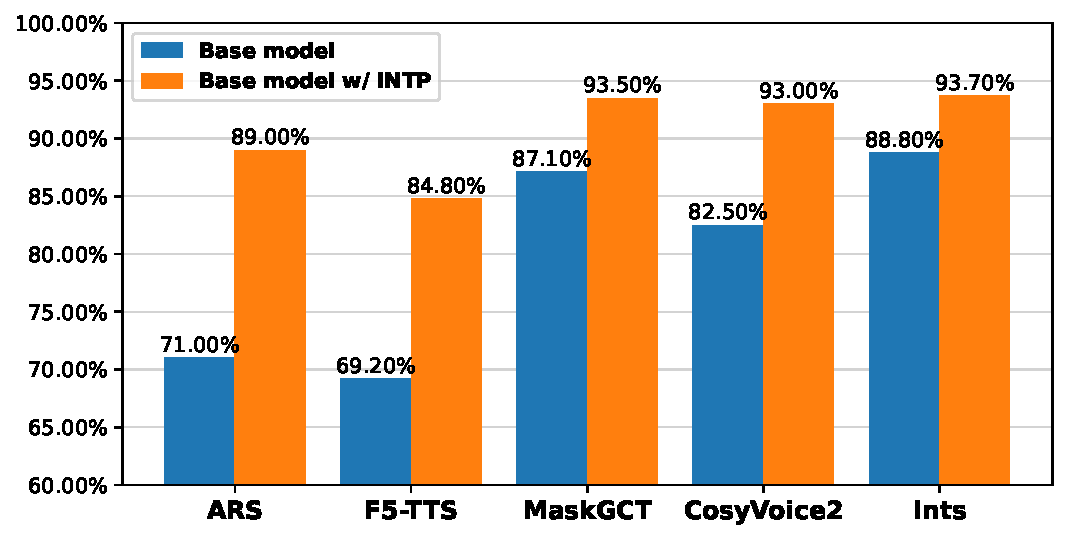
\includegraphics[width=\textwidth]{img/int_acc.pdf}
        \caption{Comparison of reading accuracy.}
        \label{fig:sub-eval-intelligibility}
        \vspace{-2mm}
    \end{subfigure}
    \hfill
    % \vfill
    \begin{subfigure}[b]{0.63\textwidth}
        \centering
        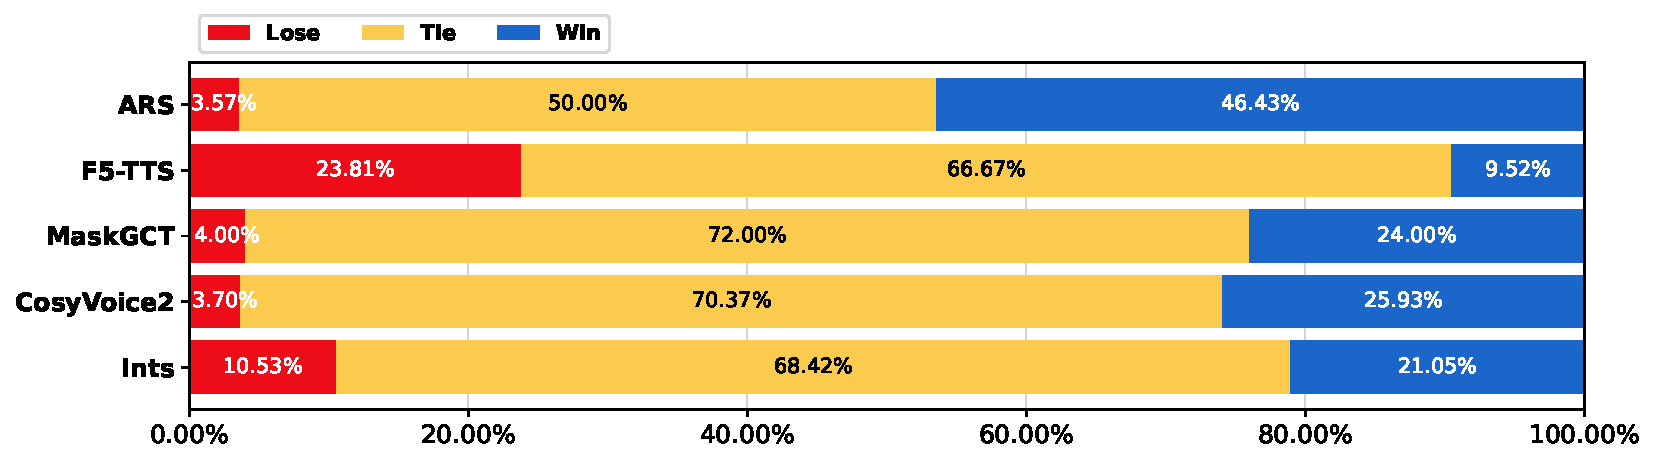
\includegraphics[width=\textwidth]{img/sim.pdf}
        \caption{Win/Lose/Tie of speaker similarity after INTP alignment.}
        \label{fig:sub-eval-similarity}
        \vspace{-2mm}
    \end{subfigure}
    \caption{Subjective evaluation of intelligibility and speaker similarity for models before and after INTP alignment.}
    \label{fig:sub-eval}
    \vspace{-4mm}
\end{figure*}


\subsection{Effect of DPO with INTP}\label{sec:expt-main}

To verify the effectiveness of DPO with INTP for existing TTS models, we conduct alignment experiments with multiple models. In addition to ARS, F5-TTS, and MaskGCT, which were used in constructing the INTP dataset, we also introduce two more powerful models in terms of intelligibility: CosyVoice 2~\cite{cosyvoice2} and Ints (Appendix~\ref{sec:appendix-detail-ins}), to validate INTP's weak-to-strong generalization capability. The experimental results are presented in Table~\ref{tab:expt-main}, including results on the objective WER, SIM, and the subjective naturalness CMOS.

We observe three key findings from Table~\ref{tab:expt-main}: (1) Across different evaluation cases, while almost all models demonstrate strong intelligibility performance in regular cases (WER < 4.0), they struggle significantly with articulatory, code-switching, and cross-lingual cases. We show some hallucinated outputs for these domains on our demo website. (2) Comparing across models, CosyVoice 2 and Ints achieves better average intelligibility performance across all cases (WER of 13.09 and 11.97), highlighting the strength of using a textual LLM as the initialization of large-scale TTS model~\cite{cosyvoice2}. (3) Through DPO with INTP, all models, including the more intelligible CosyVoice 2 and Ints that are out of the INTP distribution, show improvements in both intelligibility (WER) and naturalness (N-CMOS), and display comparable performance for speaker similarity (SIM). 

Furthermore, we randomly sample 300 samples for subjective evaluation, including assessments of reading accuracy and A/B testing of speaker similarity before and after INTP alignment (see Appendix~\ref{sec:appendix-sub-eval} for details). The results in Figure~\ref{fig:sub-eval} demonstrate that INTP alignment enhances all five models in terms of both intelligibility (higher reading accuracy in Figure~\ref{fig:sub-eval-intelligibility}) and speaker similarity (more Tie/Win percentages in Figure~\ref{fig:sub-eval-similarity}).


\subsection{Effect of Different Data within INTP}

\begin{table*}[t]
\begin{center}
\resizebox{\textwidth}{!}{
\begin{threeparttable}
    \begin{tabular}{c||rrc|rrc|rrc|rrc||rrc}
    \toprule
    \multirow{2}{*}{\textbf{Model}} & 
    \multicolumn{3}{c|}{\textbf{Regular cases}} &
    \multicolumn{3}{c|}{\textbf{Articulatory cases}} &
    \multicolumn{3}{c|}{\textbf{Code-switching cases}} &
    \multicolumn{3}{c||}{\textbf{Cross-lingual cases}} &
    \multicolumn{3}{c}{\textbf{Avg}} \\
    \cmidrule(lr){2-13} \cmidrule(lr){14-16}
     & \textbf{WER} & \textbf{SIM} & \textbf{UTMOS} & \textbf{WER} & \textbf{SIM} & \textbf{UTMOS} & \textbf{WER} & \textbf{SIM} & \textbf{UTMOS} & \textbf{WER} & \textbf{SIM} & \textbf{UTMOS} & \textbf{WER} & \textbf{SIM} & \textbf{UTMOS} \\
    \midrule 
    \rowcolor{gray!30} \multicolumn{16}{c}{\textbf{\textit{Group 1: Effect of Data across Different Text Types}}} \\
    \midrule 
    \multicolumn{1}{l||}{\textbf{ARS}~\cite{maskgct}} & 3.96 & 0.717 & 3.145 & 20.03 & 0.693 & 2.915 & 54.15 & 0.693 & 3.045 & 19.76 & 0.630 & 3.120 & 24.47 & 0.683 & 3.056 \\
    \cmidrule(lr){1-16}
    \multicolumn{1}{r||}{\textbf{w/ Regular}} & 2.45 & 0.727 & 3.200 & 17.41 & 0.706 & 3.000 & 37.52 & \textbf{0.701} & 3.110 & 9.66 & \textbf{0.638} & 3.200 & 16.76 & \textbf{0.693} & 3.128 \\
    \multicolumn{1}{r||}{\textbf{w/ Repeated}} & 2.33 & 0.725 & 3.225 & 12.88 & 0.711 & 3.050 & 39.74 & \textbf{0.701} & 3.150 & 10.96 & 0.636 & 3.235 & 16.48 & \textbf{0.693} & 3.165 \\
    \multicolumn{1}{r||}{\textbf{w/ Code-switching}} & 2.32 & \textbf{0.729} & 3.220 & 17.67 & 0.704 & 3.050 & \textbf{34.20} & 0.695 & 3.140 & 8.69 & 0.633 & 3.215 & 15.72 & 0.690 & 3.156 \\
    \multicolumn{1}{r||}{\textbf{w/ Pronunciation-perturbed}} & \textbf{2.21} & 0.720 & \textbf{3.250} & 17.76 & 0.693 & \textbf{3.075} & 35.99 & 0.687 & 3.185 & \textbf{8.24} & 0.617 & \textbf{3.285} & 16.05 & 0.679 & \textbf{3.199} \\
    \multicolumn{1}{r||}{\textbf{w/ Punctuation-perturbed}} & 2.46 & 0.722 & 3.240 & 17.35 & 0.699 & 3.020 & 42.73 & 0.694 & 3.160 & 10.94 & 0.624 & 3.255 & 18.37 & 0.684 & 3.169 \\
    \midrule
    \multicolumn{1}{r||}{\textbf{w/ INTP}} & 2.32 & 0.727 & 3.210 & \textbf{12.83} & \textbf{0.713} & 3.035 & 36.91 & 0.698 & 3.145 & 9.57 & 0.632 & 3.250 & \textbf{15.41} & 0.692 & 3.160 \\
    \midrule 
    \rowcolor{gray!30} \multicolumn{16}{c}{\textbf{\textit{Group 2: Effect of Data across Different Models}}} \\
    \midrule 
    \multicolumn{1}{l||}{\textbf{ARS}~\cite{maskgct}} & 3.96 & 0.717 & 3.145 & 20.03 & 0.693 & 2.915 & 54.15 & 0.693 & 3.045 & 19.76 & 0.630 & 3.120 & 24.47 & 0.683 & 3.056 \\ \cmidrule(lr){1-16}
    \multicolumn{1}{r||}{\textbf{w/ ARS pairs}} & 2.56 & 0.717 & 3.200 & 13.05 & 0.705 & 3.015 & 40.91 & 0.691 & 3.125 & 11.07 & 0.622 & 3.225 & 16.90 & 0.684 & 3.141 \\
    \multicolumn{1}{r||}{\textbf{w/ MaskGCT pairs}} & 2.37 & 0.724 & \textbf{3.210} & 16.85 & 0.700 & 3.010 & 37.41 & 0.692 & 3.105 & \textbf{8.83} & 0.625 & 3.200 & 16.37 & 0.685 & 3.131 \\
    \multicolumn{1}{r||}{\textbf{w/ F5-TTS pairs}} & 2.46 & 0.721 & \textbf{3.210} & 14.99 & 0.705 & \textbf{3.035} & 38.77 & 0.690 & 3.115 & 10.01 & 0.621 & 3.225 & 16.56 & 0.684 & 3.146 \\ \midrule
    \multicolumn{1}{r||}{\textbf{w/ Intra pairs}} & 2.33 & 0.721 & 3.200 & 15.29 & 0.705 & 3.015 & 37.99 & 0.687 & 3.115 & 9.36 & 0.624 & 3.200 & 16.24 & 0.684 & 3.133 \\
    \multicolumn{1}{r||}{\textbf{w/ Inter pairs}} & \textbf{2.25} & 0.726 & 3.180 & 15.42 & 0.703 & 2.965 & 38.69 & 0.697 & 3.065 & 10.61 & 0.631 & 3.170 & 16.74 & 0.689 & 3.095 \\ \midrule
    \multicolumn{1}{r||}{\textbf{w/ INTP}} & 2.32 & \textbf{0.727} & \textbf{3.210} & \textbf{12.83} & \textbf{0.713} & \textbf{3.035} & \textbf{36.91} & \textbf{0.698} & \textbf{3.145} & 9.57 & \textbf{0.632} & \textbf{3.250} & \textbf{15.41} & \textbf{0.692} & \textbf{3.160} \\
    \midrule 
    \rowcolor{gray!30} \multicolumn{16}{c}{\textbf{\textit{Group 3: Effect of Different Negative Samples}}} \\
    \midrule 
    \multicolumn{1}{l||}{\textbf{ARS}~\cite{maskgct}} & 3.96 & 0.717 & 3.145 & 20.03 & 0.693 & 2.915 & 54.15 & 0.693 & 3.045 & 19.76 & 0.630 & 3.120 & 24.47 & 0.683 & 3.056 \\ \cmidrule(lr){1-16}
    \multicolumn{1}{r||}{\textbf{w/ Regular (SFT)}$^*$} & 3.28 & 0.716 & 3.165 & 20.03 & 0.685 & 2.935 & 48.73 & 0.691 & 3.065 & 17.25 & 0.630 & 3.165 & 22.32 & 0.680 & 3.083 \\
    \multicolumn{1}{r||}{\textbf{w/ Regular$^*$}} & 2.45 & \textbf{0.727} & 3.200 & 17.41 & \textbf{0.706} & 3.000 & 37.52 & \textbf{0.701} & 3.110 & 9.66 & \textbf{0.638} & 3.200 & 16.76 & \textbf{0.693} & 3.128 \\
    \multicolumn{1}{r||}{\textbf{w/ Pronunciation-perturbed}$^*$} & \textbf{2.21} & 0.720 & \textbf{3.250} & 17.76 & 0.693 & \textbf{3.075} & \textbf{35.99} & 0.687 & \textbf{3.185} & \textbf{8.24} & 0.617 & \textbf{3.285} & \textbf{16.05} & 0.679 & \textbf{3.199} \\
    \multicolumn{1}{r||}{\textbf{w/ Punctuation-perturbed}$^*$} & 2.46 & 0.722 & 3.240 & \textbf{17.35} & 0.699 & 3.020 & 42.73 & 0.694 & 3.160 & 10.94 & 0.624 & 3.255 & 18.37 & 0.684 & 3.169 \\
    \bottomrule
    \end{tabular}
    \begin{tablenotes}
        \item[*] The positive samples in these four experiments are identical. \textbf{w/ Regular (SFT)} refers to supervised fine-tuning using positive samples only, excluding negative samples. \textbf{w/ Regular} employs WER-based negative samples, while the other two utilize our proposed human-guided negative samples.
    \end{tablenotes}
\end{threeparttable}
}
\caption{Effect of different data within INTP for ARS.}
\label{tab:expt-abs-total}
\end{center}
\end{table*}

To investigate the impact of different distributions within INTP, we conduct ablation studies from multiple perspectives. In Table~\ref{tab:expt-abs-total}, we present three groups of experiments on ARS: the effect of data across different text types, across different models, and the effect of different negative samples. Additional results, including the effect of data across different languages are provided in Appendix~\ref{sec:appendix-more-results}.

We observe three key findings from Table~\ref{tab:expt-abs-total}: (1) Group 1 demonstrates that different scenarios require customized post-training data. For instance, repeated data proves particularly effective for articulatory cases, while pronunciation-perturbed data significantly improves pronunciation accuracy and WER in cross-lingual cases (see our demo website for details). Moreover, utilizing data from multiple scenarios (i.e., the complete INTP) yields the best overall improvements. (2) Group 2 reveals that model improvement can be achieved through alignment using synthetic data, regardless of whether it's generated by the model itself or other models. Besides, the intra-pairs and inter-pairs are complementary for model improvements. (3) Group 3 shows that using only positive samples from INTP for supervised fine-tuning (SFT) can already improve quality. Building upon this, incorporating negative samples for preference learning leads to even more substantial gains. 

% Furthermore, the results from Group 3 validate the effectiveness of our proposed human-guided negative samples.

\subsection{Iterative Intelligibility Alignment}\label{sec:iterative-align}

\begin{table*}[t]
\vspace{-3mm}
\begin{center}
\begin{threeparttable}
    \resizebox{\textwidth}{!}{
    \begin{tabular}{c|c||rcc|rcc|rcc|rcc||rcc}
    \toprule
    \multirow{2}{*}{\textbf{Model}} & 
    \multirow{2}{*}{\textbf{Preference Data}} & 
    \multicolumn{3}{c|}{\textbf{Regular cases}} &
    \multicolumn{3}{c|}{\textbf{Articulatory cases}} & 
    \multicolumn{3}{c|}{\textbf{Code-switching cases}} &
    \multicolumn{3}{c||}{\textbf{Cross-lingual cases}} &
    \multicolumn{3}{c}{\textbf{Avg}} \\
    \cmidrule(lr){3-14} \cmidrule(lr){15-17}
     & & \textbf{WER} & \textbf{SIM} & \textbf{UTMOS} & \textbf{WER} & \textbf{SIM} & \textbf{UTMOS} & \textbf{WER} & \textbf{SIM} & \textbf{UTMOS} & \textbf{WER} & \textbf{SIM} & \textbf{UTMOS} & \textbf{WER} & \textbf{SIM} & \textbf{UTMOS} \\
    \midrule
    \textbf{Ints} & - 
        & 3.14 & 0.688 & 3.175 
        & 12.08 & 0.666 & 3.025 
        & 22.88 & 0.646 & 3.045 
        & 9.78 & 0.572 & 3.150 
        & 11.97 & 0.643 & 3.099 \\
    \textbf{Ints v1} & \textbf{INTP} 
        & 2.36 & 0.686 & 3.205 
        & 9.38 & 0.664 & 3.060 
        & 13.80 & 0.642 & 3.125 
        & 6.28 & 0.571 & 3.230 
        & 7.96 & 0.641 & 3.155 \\
    \textbf{Ints v2} & \textbf{Ints v1 generated} 
        & 2.21 & 0.686 & 3.210 
        & 8.48 & 0.660 & 3.085 
        & 12.33 & 0.643 & 3.140 
        & 5.40 & 0.567 & 3.250 
        & 7.10 & 0.639 & 3.171 \\
    \bottomrule
    \end{tabular}
    }
\end{threeparttable}
\caption{Iterative Preference Alignment for Ints.}
\label{tab:data_flywheel}
\end{center}
\vspace{-3mm}
\end{table*}

% Furthermore, we explore how to establish an \textit{iterative} preference alignment, i.e., data and model flywheel~\cite{RLHF-anthoropic,llama3,iterative-dpo}. Taking Ints as an example, we refer to the version of Ints that has undergone alignment with INTP as Ints v1. Subsequently, we reuse the prompts and texts from INTP. For a given case, we regenerate multiple samples using Ints v1 and select positive and negative pairs from these samples. Finally, we perform another round of alignment training on Ints v1 using the pairs generated by Ints v1, with the resulting model denoted as Ints v2. The results of the iterative alignment are shown in Table~\ref{tab:data_flywheel}. The further iteration with Ints v2 yields additional improvements, demonstrating enhanced intelligibility across all scenarios, ultimately achieving the lowest average WER 7.104 and highest average UTMOS 3.171. This demonstrates that the preference data generated by a better-aligned model can still lead to subsequent alignment.

Furthermore, we explore how to establish an \textit{iterative} preference alignment, i.e., data and model flywheel~\cite{RLHF-anthoropic,llama3,iterative-dpo}. This approach aligns with the online reinforcement learning (RL) framework \citet{li2023rema4}.  We investigate two rounds of alignment based on Ints, where Ints v1 (INTP-aligned model) is used to generate new preference data for training Ints v2, following a similar \textit{cadence} of data collection as~\cite{RLHF-anthoropic}. To prepare Ints v1 generated preference data, we sample a challenging prompt subset from INTP and adopt the same pipeline as INTP to construct preference pairs (see Appendix~\ref{sec:appendix-ints-training-data} for details). The results of this iterative alignment are shown in Table~\ref{tab:data_flywheel}. We can observe that compared to Ints v1, Ints v2 yields additional improvements across all scenarios, which demonstrates that effectiveness of iterative alignment. However, we observe that the magnitude of improvement in the second round is notably smaller than the first round. We suspect this indicates that the upper bound of iterative alignment is largely determined by the base model's inherent capabilities, suggesting future research should focus on base models with higher potential.

\section{Conclusion}

% In this work, we propose a preference alignment framework to enhance intelligibility in zero-shot TTS systems, especially in challenging scenarios such as hard-to-pronounce texts, code-switching, and cross-lingual synthesis. Central to our approach is the INTP dataset, a synthetic intelligibility preference dataset comprising about 250K pairs that span diverse scenarios and domains. We adapt DPO for various TTS architectures, which significantly improves both intelligibility and naturalness. Additionally, we introduce the Ints model, an intelligibility-enhanced speech model initialized from a textual LLM, which also benefits from intelligent enhancements with INTP alignment.

% In this work, we thoroughly analyze the intelligibility issues of modern zero-shot TTS systems across diverse domains, especially in hard-to-pronounce texts, code-switching, and cross-lingual synthesis. We propose to address these challenges using preference alignment with our newly constructed INTP dataset. INTP contains about 250K pairs with three different preference determination methods: model's self-comparison based intra pairs, cross-model comparison based inter pairs, and human-guided perturbed pairs. Moreover, we employ DPO and design its special extensions, which significantly improve both intelligibility and naturalness across various TTS architectures using INTP. Finally, we demonstrate INTP's weak-to-strong generalization capability and establish an iterative preference alignment flywheel with more powerful base models, highlighting the broad potential of our proposed alignment framework in future speech generation research.

In this work, we focus on the intelligibility issues of modern zero-shot TTS systems across diverse domains, especially in hard-to-pronounce texts, code-switching, and cross-lingual synthesis. We propose to address these challenges using preference alignment with our newly constructed INTP dataset, which contains diverse preference pairs determined through model self-comparison, cross-model comparison, and human guidance. We employ DPO and design  special extensions to significantly improve various TTS architectures, while demonstrating INTP's weak-to-strong generalization capability and establishing an iterative preference alignment flywheel with more powerful base models.

% \clearpage


\section*{Limitations}

While our approach demonstrates significant improvements in zero-shot TTS intelligibility across diverse domains, several limitations remain. Although INTP covers multiple challenging scenarios, it may not fully capture all edge cases, such as specialized jargon or rare language pairs. Future work could expand to more low-resource languages and niche domains. Besides, constructing INTP and conduct alignment experiments on large models like Ints require substantial computational resources, potentially limiting accessibility.

\section*{Potential Risks}

The proposed method introduces several risks that warrant consideration. Enhanced TTS systems could be exploited to generate deceptive content (e.g., deepfake audio), posing ethical challenges. Robust safeguards and watermarking mechanisms are critical for deployment. While INTP uses public datasets, real-world applications may risk incorporating sensitive or copyrighted speech data, requiring strict governance protocols.

\section*{Acknowledgment}
This work is partially supported by the NSFC under Grant 62376237, Shenzhen Science and Technology Program ZDSYS20230626091302006, and Shenzhen Research Institute of Big Data (Internal Project Fund, Grant No. T00120230002). We appreciate Yushun Zhang and the anonymous reviewers for their insightful comments and suggestions.

% Bibliography entries for the entire Anthology, followed by custom entries
% \bibliography{anthology,custom}
% Custom bibliography entries only
\bibliography{custom}

% \clearpage
\appendix

\section{Construction Details of INTP}

\subsection{Prompt Construction}
\label{sec:appendix-prompt-construction}

We construct English and Chinese prompt data, both based on the Emilia-Large dataset~\cite{emilia,emilia-large}, which contains diverse real-world speech data across various topics, recording scenarios, and speaking styles. 

\paragraph{Reference Speech}

We perform stratified sampling on Emilia-Large's speech data based on its metadata such as topics and tags to cover diverse acoustic conditions. Considering the memory constraints of existing zero-shot TTS models during inference, we only select samples with durations not exceeding 12 seconds.

\paragraph{Target Text}\label{sec:appendix-prompt-target-text-construction}
Similarly to reference speech, we perform stratified sampling based on Emilia-Large's metadata to cover diverse semantic topics. We select speech samples with durations between 5 and 22 seconds, and use their corresponding textual transcriptions as the target text data source.

We utilize DeepSeek V3~\cite{deepseek-r1} to preprocess the sampled textual transcriptions, such as typo correction and punctuation mark normalization, and use the processed text as regular text in INTP. Specifically, we use the following instruction for DeepSeek V3 to conduct text preprocessing:

\begin{promptbox}
\textit{\textbf{System Prompt:} }\\
I obtained a text from an audio file based on some ASR models. Please help me clean it up (e.g., correct typos, add proper punctuation marks, and make the sentences semantically coherent). Note: (1) You can modify, add, or replace words that better fit the context to ensure semantic coherence. (2) Please only return the cleaned-up result without any explanation.

\medskip \textit{\textbf{User Prompt (Example):} }\\
a panda eats shoes and leaves

\medskip \textit{\textbf{System Output (Example):} }\\
A panda eats shoots and leaves.
\end{promptbox}

Furthermore, we employ DeepSeek V3 to transform the regular text into different types. To generate Chinese-English-mixed code-switching texts:

\begin{promptbox}
\textit{\textbf{System Prompt:} }\\
\begin{CJK*}{UTF8}{gbsn}
    请你把这句话，转换成一个中文、英文混合的~code-switching~版本。注意：你只需要返回给我转换后的结果，不需要任何解释。
\end{CJK*}

\medskip \textit{\textbf{User Prompt (Example):} }\\
A panda eats shoots and leaves.

\medskip \textit{\textbf{System Output (Example):} }\\
\begin{CJK*}{UTF8}{gbsn}
    熊猫吃~shoots~和~leaves。
\end{CJK*}

\end{promptbox}

To generate punctuation-perturbed texts:

\begin{promptbox}
\textit{\textbf{System Prompt:} }\\
\begin{CJK*}{UTF8}{gbsn}
    假设你是一个~Text To Speech (TTS)~领域的专家，现在，让我们对一个~TTS~系统进行攻击。具体地：我输入一个文本，请你修改这条文本里面的若干词语，从而使~TTS~系统更容易出错。例如：你可以修改为把某些字修改为容易读错的形近字、把多音字做替换，等等，但你不要增加和删除原有的文本。注意：你只需要返回给我转换后的结果，不需要任何解释。\\
    
    例子1: \\
    【我的输入】我今天很高兴\\
    【你的输出】窝锦添狠搞醒\\

    例子2: \\
    【我的输入】目前，爱心人士正在种作寄养的小猫已经五个月大了。而本人的种作寄养申请单需要进一步审核。为了避免小猫多次转手，治疗者们对小猫的种作寄养提出了严格要求：申请人需年满二十三岁。\\
    【你的输出】幕前，爱信人士正在重作寄扬的削猫已经伍个月大了。而本人的重作寄扬神情但需要进一步审核。为了闭面削猫多次转售，治理者们对削猫的重作寄扬提出了阉割要求：申情人需年慢贰拾叁岁。\\

    例子3: \\
    【我的输入】And the idea of standing all by himself in a crowded market, to be pushed and hired by some big, strange farmer, was very disagreeable. Why not sing that high note and grow potatoes?\\
    【你的输出】And the eye dear of standing awl bye himself in a crowd dead market, two bee pushed and high red buy sum big, strange far mer, was vary dis agreeable. Y knot sing that hi note and grow poe eight toes?\\
\end{CJK*}

\medskip \textit{\textbf{User Prompt (Example):} }\\
A panda eats shoots and leaves.

\medskip \textit{\textbf{System Output (Example):} }\\
A pan duh eights shots n leafs.

\end{promptbox}

To generate repeated text and punctuation-perturbed text, we leverage DeepSeek V3 to create executable Python scripts that implement rule-based word repetition and random punctuation modification. These scripts will be included in our future open-source repository.

\paragraph{Combination between Speech and Text}

Based on the language of reference speech and target text data, we design four balanced combination categories: monolingual combinations (\textit{en2en} and \textit{zh2zh}) and cross-lingual combinations (\textit{zh2en} and \textit{en2zh}), where \textit{zh2en} denotes Chinese reference speech with English target text, and similarly for others. For each text type shown in Table~\ref{tab:intp-stats} (Regular, Repeated, Code-Switching, Pronunciation-perturbed, and Punctuation-perturbed), we construct 12K prompts.

\subsection{Model Selection}\label{sec:appendix-model-selection}

\begin{itemize}[itemsep=0ex,leftmargin=2ex]
    \item \textbf{ARS}~\cite{maskgct}: We use the original checkpoint (pre-trained on Emilia) provided by the authors.
    \item \textbf{F5-TTS}~\cite{f5tts}: We use the officially released checkpoint\footnote{\href{https://huggingface.co/SWivid/F5-TTS}{https://huggingface.co/SWivid/F5-TTS}} for INTP data generation.
    \item \textbf{MaskGCT}~\cite{maskgct}: We use the officially released checkpoint\footnote{\href{https://huggingface.co/amphion/MaskGCT}{https://huggingface.co/amphion/MaskGCT}}~\cite{amphion,amphion_v0.2} for INTP data generation.
\end{itemize}

In addition to these three models used for INTP construction, we also investigate INTP's effectiveness on \textbf{CosyVoice 2} and \textbf{Ints}. For CosyVoice 2, we conduct alignment experiments using its officially released checkpoint\footnote{\href{https://github.com/FunAudioLLM/CosyVoice}{https://github.com/FunAudioLLM/CosyVoice}} as the base model. Details of the pre-trained models of Ints are provided in Appendix~\ref{sec:appendix-detail-ins}.


\subsection{Preference Pairs Construction}\label{sec:appendix-preference-pairs}

\subsubsection{Intra Pair}\label{sec:appendix-intp-intra-pair}

For each model and prompt, we perform five samplings and construct intra pairs based on their WER comparisons. To maximize the performance gap between positive and negative samples, we employ two strategies. First, we use diverse hyperparameters during the five generations to increase sample diversity, selecting the generation with the lowest WER as positive samples and the highest WER as negative samples. Second, we apply a threshold to filter out pairs where the WER gap between positive and negative samples is less than 6.0.

Specifically, for ARS's five samplings, we set top k to 20 and top p to 1.0, while using different temperatures of 0.4, 0.6, 0.8, 1.0, and 1.2. For F5-TTS and MaskGCT, we use the generated speech target duration as the sampling hyperparameter. Denoting the ``ground truth'' duration\footnote{Since we use Emilia-Large's transcription data as target text in our prompt construction process (Appendix~\ref{sec:appendix-prompt-target-text-construction}), we refer to the original speech duration corresponding to this transcription as the ``ground truth'' duration.} as $d$, we employ five different duration parameters: 0.8$d$, 0.9$d$, 1.0$d$, 1.1$d$, and 1.2$d$.

\subsubsection{Inter Pair}\label{sec:appendix-intp-inter-pair}

We construct inter pairs based on the intra pairs established in Appendix~\ref{sec:appendix-intp-intra-pair}. For a given prompt, we denote model A's intra pair as $(y^w_A, y^l_A)$ and model B's intra pair as $(y^w_B, y^l_B)$. We construct inter pairs through three types of comparisons: between $y^w_A$ and $y^w_B$, between $y^w_A$ and $y^l_B$, and between $y^l_A$ and $y^w_B$. Note that we exclude comparisons between $y^l_A$ and $y^l_B$ to ensure high quality of positive samples. We apply the same WER threshold as in Appendix~\ref{sec:appendix-intp-intra-pair} to filter out pairs with small performance gaps.

\subsubsection{Perturbed Pair}\label{sec:appendix-intp-perturbed-pair}

The instructions used to prompt DeepSeek V3 for obtaining pronunciation-perturbed and punctuation-perturbed texts are shown in Appendix~\ref{sec:appendix-prompt-target-text-construction}. Specifically, we only use data from INTP's regular text domain to construct perturbed pairs.

\subsection{Human Verification}\label{sec:appendix-intp-human-verficiation}

\begin{table}[t]
\begin{center}
\resizebox{0.8\columnwidth}{!}{%
\begin{threeparttable}
    \begin{tabular}{ccccc}
        \toprule
         \makecell[c]{\textbf{A+2}} & \makecell[c]{\textbf{A+1}} & \makecell[c]{\textbf{Tie}} & \makecell[c]{\textbf{B+1}} & \makecell[c]{\textbf{B+2}} \\ \midrule
         10.9\% & 29.0\% & 15.0\% & 32.4\% & 12.6\% \\
         \bottomrule
    \end{tabular}
    \begin{tablenotes}
        \footnotesize{
            \item[*] For each pair, we present the two samples to human raters in random order, labeled as A and B. A+2 indicates that sample A's naturalness is significantly better than B, while A+1 indicates that sample A is moderately better than B, similar for B+2 and B+1. Tie indicates no perceptible difference.
        }
    \end{tablenotes}
\end{threeparttable}
}
\caption{Human naturalness preference for 1,000 pairs from INTP regular text domain.}
\label{tab:human-naturalness-verify}
\end{center}
\end{table}

\begin{table}[t]
\begin{center}
\resizebox{\columnwidth}{!}{%
\begin{threeparttable}
    \begin{tabular}{c|ccc}
        \toprule
         & \textbf{\makecell[c]{Naturalness\\Winner}} & \textbf{\makecell[c]{Naturalness\\Tie}} & \textbf{\makecell[c]{Naturalness\\Loser}} \\ \midrule
         \textbf{INTP winner} & 72\% & 15\% & 13\% \\
         % \textbf{INTP loser} & 13\% & 15\% & 72\% \\
         \bottomrule
    \end{tabular}
\end{threeparttable}
}
\caption{Agreement between INTP preference and human naturalness preference.}
\label{tab:human-naturalness-compare-wer}
\end{center}
\end{table}

In Section~\ref{sec:intp-human-verify}, we evaluated INTP's alignment with human intelligibility perception. In this section, we investigate the alignment between INTP and human naturalness preferences. Specifically, we design a \textbf{naturalness preference} annotation task (Appendix~\ref{sec:appendix-sub-eval}). We randomly sample 1,000 pairs from INTP's regular text domain for human annotation, with results shown in Table~\ref{tab:human-naturalness-verify} and~\ref{tab:human-naturalness-compare-wer}. The results reveal two key findings: First, 85\% of INTP pairs exhibit distinguishable naturalness preferences (Tie rate of 15\% in Table~\ref{tab:human-naturalness-verify}). Additionally, INTP's preference determination shows strong agreement with human naturalness preferences (72\% agreement rate between INTP winners and naturalness winners in Table~\ref{tab:human-naturalness-compare-wer}). These results suggest that INTP can also serve as a foundation dataset for naturalness preference alignment in future research.

\section{Details of the Derivation}\label{sec:appendix-derivation}


\subsection{DPO for AR Models}\label{sec:appendix-derivation-ar}

Starting from Equation~\ref{eq:rl_obj}, \citet{dpo} demonstrate that the optimization problem admits a closed-form solution. Specifically, the optimal policy \( p_\theta^*(y | x) \) that maximizes the RL objective is given by:
\begin{equation}
    {\small
    \begin{aligned}
p_\theta^*(y | x) = \frac{1}{Z(x)} p_{\text{ref}}(y | x) \exp\left(\frac{1}{\beta} r(x, y)\right),
    \end{aligned}
    }
\label{eq:optimal_policy}
\end{equation}
where \( Z(x) \) is the partition function ensuring normalization. This establishes a direct relationship between the reward function and the policy:
\begin{equation}
    {\small
    \begin{aligned}
    r(x, y) = \beta \log \frac{p_\theta^*(y | x)}{p_{\text{ref}}(y | x)} + \beta \log Z(x).
    \end{aligned}
    }
\label{eq:reward_expression}
\end{equation}
Substituting this reward expression (Equation~\ref{eq:reward_expression}) into the reward modeling loss function (Equation~\ref{eq:reward_model}) leads the DPO loss (Equation~\ref{eq:dpo_ar}), which we represent here as:
\[
    {\small
    \begin{aligned}
\mathcal{L}_\text{DPO} = -\mathbb{E}_{\mathcal{D}} \left[ \log \sigma\left( \beta \left( \log \tfrac{p_\theta(y_w | x)}{p_{\text{ref}}(y_w | x)} - \log \tfrac{p_\theta(y_l | x)}{p_{\text{ref}}(y_l | x)} \right) \right) \right].
    \end{aligned}
    }
\]

\subsection{DPO for Flow-Matching Models}\label{sec:appendix-derivation-fm}

Starting from Equation~\ref{eq:rl_obj_fm}, which we represent here as:
\[{\small
\begin{aligned}
\max_{p_\theta} & \mathbb{E}_{y_1 \sim p_\theta(y_1|x), t, x}[r(y_1,x)] \\
& - \beta \mathbb{D}_{\text{KL}}[p_\theta(y_1|y_t,t,x) \| p_{\text{ref}}(y_1|y_t,t,x)].
\end{aligned}
}\]
Similar to the derivation in DPO~\cite{dpo} and~\citet{wallace2024diffusion}, we obtain the closed-form solution for the optimal policy as:
\begin{equation}
    {\scriptsize
    \begin{aligned}
    p_\theta^*(y_1 | y_t, t, x) = \frac{1}{Z(y_t, t, x)} p_{\text{ref}}(y_1 | y_t, t, x) \exp\left(\frac{1}{\beta} r(y_1, x)\right),
    \end{aligned}
    }
\end{equation}
where \( Z(y_t, t, x) \) is the partition function ensuring normalization. We can then express the reward model \( r(y_1, x) \) as:
\begin{equation}
    {\small
    \begin{aligned}
    r(y_1, x) = \beta \log \frac{p_\theta^*(y_1 | y_t, t, x)}{p_{\text{ref}}(y_1 | y_t, t, x)} + \beta \log Z(y_t, t, x).
    \end{aligned}
    }
    \label{eq:reward_expression_fm}
\end{equation}
Similarly, substituting this reward expression (Equation~\ref{eq:reward_expression_fm}) into the reward modeling loss function (Equation~\ref{eq:reward_model}) leads to the DPO loss for OT-FM (Equation~\ref{eq:dpo-fm}), which we represent here:
\[
{\scriptsize
\begin{aligned}
& \mathcal{L}_{\text{DPO-FM}} = -
\mathbb{E}_{(y_1^w, y_1^l, x) \sim \mathcal{D}, t} \\
& \log \sigma \left( \beta \left( \log \frac{p_\theta(y_1^w|y_t^w,t,x)}{p_{\text{ref}}(y_1^w|y_t^w,t,x)}
- \log \frac{p_\theta(y_1^l|y_t^l,t,x)}{p_{\text{ref}}(y_1^l|y_t^l,t,x)} \right) \right).
\end{aligned}
}
\]
Reviewing the training objective of OT-FM (Equation~\ref{eq:obj_fm}), we find that it is equivalent to fitting a Gaussian likelihood. In other words, the induced likelihood can be interpreted as:
\[
{\small
\begin{aligned}
p_\theta(y_1 \mid y_t, t, x) \propto \exp\!\left(-\frac{1}{\beta}\left\|v_\theta(y_t,t,x) - (y_1-y_0)\right\|_2^2\right),
\end{aligned}
}
\]
similarly, for the reference policy, we have:
\[
{\small
\begin{aligned}
p_{\mathrm{ref}}(y_1 \mid y_t, t, x) \propto \exp\!\left(-\frac{1}{\beta}\left\|v_{\mathrm{ref}}(y_t,t,x) - (y_1-y_0)\right\|_2^2\right).
\end{aligned}
}
\]
Here, \(\beta\) serves as an inverse temperature (or noise variance), and the normalization constants cancel out when taking the ratio.
By taking the logarithm of the ratio between the learned policy and the reference policy, we obtain:
\[
{\small
\begin{aligned}
\log\frac{p_\theta(y_1\mid y_t,t,x)}{p_{\mathrm{ref}}(y_1\mid y_t,t,x)} = & -\frac{1}{\beta} \Bigl( \|v_\theta(y_t,t,x) - (y_1-y_0)\|_2^2 \\
& - \|v_{\mathrm{ref}}(y_t,t,x) - (y_1-y_0)\|_2^2\Bigr).
\end{aligned}
}
\]
Multiplying both sides by \(\beta\) results in:
\[
{\small
\begin{aligned}
\beta\log\frac{p_\theta(y_1\mid y_t,t,x)}{p_{\mathrm{ref}}(y_1\mid y_t,t,x)} = & -\Bigl( \|v_\theta(y_t,t,x) - (y_1-y_0)\|_2^2 \\
& - \|v_{\mathrm{ref}}(y_t,t,x) - (y_1-y_0)\|_2^2 \Bigr).
\end{aligned}
}
\]
By substituting the log-ratio formulation into Equation~\ref{eq:dpo-fm}, we can transform the DPO loss for OT-FM into a form related to the velocity, as shown in Equation~\ref{eq:dpo-fm-velocity}, which is represented as:
\[
{\tiny
\begin{aligned}
& \mathcal{L}_{\text{DPO-FM}} = -\mathbb{E}_{(y_1^w, y_1^l, x) \sim \mathcal{D}, t} \log \sigma \Big( -\beta \\
& \Big( \left\| v_\theta(y^w_t, t, x) - (y_1^w - y_0^w) \right\|_2^2
- \left\| v_\text{ref}(y^w_t, t, x) - (y_1^w - y_0^w) \right\|_2^2 \Big) \\
& - \Big( \left\| v_\theta(y^l_t, t, x) - (y_1^l - y_0^l) \right\|_2^2
- \left\| v_\text{ref}(y^l_t, t, x) - (y_1^l -y_0^l) \right\|_2^2 \Big) \Big).
\end{aligned}
}
\]

\subsection{DPO for Masked Generative Models}\label{sec:appendix-derivation-mgm}

% Add to appendix
% We extend DPO for MGM. Let \(p_\theta(y_0 \mid y_t, x)\) denote the policy to optimize, and \(p_{\text{ref}}(y_0 \mid y_t, x)\) the reference policy. We rewrite the RL objective for MGM as:
% \begin{equation}
% {\small
% \begin{aligned}
% \max_{p_\theta} \quad & \mathbb{E}_{y_0 \sim p_\theta(y_0|x), t, x} \left[ r(y_0, x) \right] \\
% & - \beta \mathbb{D}_{\text{KL}} \left[ p_\theta(y_0|y_t,x) \,\|\, p_{\text{ref}}(y_0|y_t,x) \right],
% \end{aligned}
% }
% \end{equation}
% Following the DPO derivation, we reparameterize the reward in terms of the policy and reference log-probabilities. Given the preference dataset \(\mathcal{D} = \{(y_0^w, y_0^l, x)\}\), the DPO loss for MGM becomes:  
% \begin{equation}
% {\scriptsize
% \begin{aligned}
% & \mathcal{L}_{\text{DPO-MGM}} = -\mathbb{E}_{(y^w, y^l, x) \sim \mathcal{D}, t}  \\
% & \log \sigma \left( \beta \left( \log \frac{p_\theta(y^w_0|y^w_t,x)}{p_{\text{ref}}(y^w_0|y^w_t,x)}
%  - \log \frac{p_\theta(y^l_0|y^l_t,x)}{p_{\text{ref}}(y^l_0|y^l_t,x)} \right) \right).
% \end{aligned}
% }
% \end{equation}
% Here, \(y^w_t\) and \(y^l_t\) are masked versions of \(y^w_0\) and \(y^l_0\) generated via the mask schedule \(\gamma(t)\). Note that $p_\theta(y_0|y_t,x)$ corresponds to the sum of the log-probabilities of the unmasked tokens in the context of MGM.

Similar to flow-matching, let \(p_\theta(y_0 \mid y_t, x)\) denote the policy to be optimized, and \(p_{\text{ref}}(y_0 \mid y_t, x)\) the reference policy. We can rewrite the RL objective for MGM as follows:
\begin{equation}
{\small
\begin{aligned}
\max_{p_\theta} \quad & \mathbb{E}_{y_0 \sim p_\theta(y_0|x), t, x} \left[ r(y_0, x) \right] \\
& - \beta \mathbb{D}_{\text{KL}} \left[ p_\theta(y_0|y_t,x) \,\|\, p_{\text{ref}}(y_0|y_t,x) \right].
\end{aligned}
}
\end{equation}
We can also derive the closed-form solution for the optimal policy:
\begin{equation}
{\small
\begin{aligned}
p_\theta^*(y_0 | y_t, x) = \frac{1}{Z(y_t, x)} p_{\text{ref}}(y_0 | y_t, x) \exp\left(\frac{1}{\beta} r(y_0, x)\right),
\end{aligned}
}
\end{equation}
and express the reward model as follows:
\begin{equation}
{\small
\begin{aligned}
r(y_0, x) = \beta \log \frac{p_\theta^*(y_0 | y_t, x)}{p_{\text{ref}}(y_0 | y_t, x)} + \beta \log Z(y_t, x),
\end{aligned}
}
\label{eq:reward_expression_mgm}
\end{equation}
where \( Z(y_t, x) \) is the partition function ensuring normalization.
Also, substituting this reward expression (Equation~\ref{eq:reward_expression_mgm}) into the reward modeling loss function (Equation~\ref{eq:reward_model}) leads to the DPO loss for MGM:
\begin{equation}
{\scriptsize
\begin{aligned}
& \mathcal{L}_{\text{DPO-MGM}} = -\mathbb{E}_{(y^w, y^l, x) \sim \mathcal{D}, t}  \\
& \log \sigma \left( \beta \left( \log \frac{p_\theta(y^w_0|y^w_t,x)}{p_{\text{ref}}(y^w_0|y^w_t,x)}
 - \log \frac{p_\theta(y^l_0|y^l_t,x)}{p_{\text{ref}}(y^l_0|y^l_t,x)} \right) \right).
\end{aligned}
}
\end{equation}
Here, \(y^w_t\) and \(y^l_t\) are masked versions of \(y^w_0\) and \(y^l_0\) generated via the mask schedule \(\gamma(t)\). Note that $p_\theta(y_0|y_t,x)$ corresponds to the sum of the log-probabilities of the unmasked tokens in the context of MGM.

\section{Ints: Intelligibility-enhanced Speech Language Model}\label{sec:appendix-detail-ins}

Ints is an \underline{int}elligibility-enhanced \underline{s}peech language model. 
% It follows a two-stage generation architecture like previous studies~\cite{seedtts,cosyvoice,maskgct,vevo}: in the first stage, it uses an AR model to generate discrete speech tokens, while in the second stage, it employs a flow matching model to generate mel-spectrograms. We use the first-layer tokens from DualCodec~\cite{dualcodec} as the modeling target for the first stage of Ints, due to its efficient compression representation (12.5Hz tokens for 24kHz speech) and rich semantic information. We highlight that our first-stage AR model is directly \textbf{initialized from a textual LLM} while extending the vocabulary to include speech tokens. Specifically, in this work, we use the 3.8B \texttt{Phi-3.5-mini-instruct}~\cite{phi3}, motivated by scaling up model size and leveraging the rich textual semantic knowledge~\cite{naturalspeech3,cosyvoice2,llasa}. We format the input as a text-to-speech instruction concatenated with speech tokens (see Appendix~\ref{sec:appendix-detail-ins} for details). 
It follows a two-stage generation paradigm like~\cite{seedtts, cosyvoice, maskgct}: in the first stage, it uses an AR model to generate discrete speech tokens, while in the second stage, it employs a flow matching model to generate mel-spectrograms from speech tokens. We use the first-layer tokens from DualCodec~\cite{dualcodec} as the modeling target for the first stage of Ints, due to its efficient compression representation (12.5Hz tokens for 24kHz speech) and rich semantic information. Particularly, the first-stage AR model is directly \textbf{initialized from a large language model} while extending the vocabulary to include speech tokens. The codebook size of speech tokens is 16,384. Specifically, in this work, we use the 3.8B \texttt{Phi-3.5-mini-instruct}\footnote{\href{https://huggingface.co/microsoft/Phi-3.5-mini-instruct}{https://huggingface.co/microsoft/Phi-3.5-mini-instruct}}~\cite{phi3}, motivated by scaling up model size and leveraging the rich textual semantic knowledge.

\subsection{TTS Instruction Design}

We format the input as a text-to-speech instruction concatenated with speech tokens. The input sequence is represented as: 
\[
\left[\boldsymbol{I}, \boldsymbol{T}, <|\text{startofspeech}|>, \boldsymbol{S}, <|\text{endofspeech}|> \right]
\]
where \(\boldsymbol{I}\) is the instruction prefix (e.g., ``Please speak the following text out loud''), and \(\boldsymbol{T}\) and \(\boldsymbol{S}\) denote the text and speech token sequences, respectively. The special tokens \(<|\text{startofspeech}|>\) and \(<|\text{endofspeech}|>\) mark the boundaries of the speech token sequence.

During the inference stage for zero-shot TTS, the input sequence is represented as:
\[
\left[\boldsymbol{I}, \boldsymbol{T}_{\text{prompt}}, \boldsymbol{T}_{\text{target}}, <|\text{startofspeech}|>, \boldsymbol{S}_{\text{prompt}} \right]
\]
to generate the target speech tokens \(\boldsymbol{S}_{\text{target}}\). Here, \(\boldsymbol{T}_{\text{prompt}}\), \(\boldsymbol{T}_{\text{target}}\), \(\boldsymbol{S}_{\text{prompt}}\) are placeholders for the prompt text, target text, and prompt speech tokens, respectively.

\subsection{Training data}\label{sec:appendix-ints-training-data}

We pre-train Ints on Emilia~\cite{emilia}, which consists of about 100K hours of multilingual data. Following this, we use INTP alignment to obtain Ints v1. Ints v1 is then used to generate new preference data, which are employed to train Ints v2 for iterative alignment. We select prompts from the repeated and code-switching samples of INTP, which can be considered a more challenging subset of prompts. For each prompt, we use the same INTP intra-pair pipeline in Appendix~\ref{sec:appendix-intp-intra-pair} to construct preference pairs.

\begin{table*}[t]
\begin{center}
\resizebox{\textwidth}{!}{
\begin{threeparttable}
    \begin{tabular}{c||rrc|rrc|rrc|rrc||rrc}
    \toprule
    \rowcolor{gray!30} \multicolumn{16}{c}{\textbf{\textit{On English Evaluation Samples}}} \\
    \midrule 
    \multirow{2}{*}{\textbf{Model}} & 
    \multicolumn{3}{c|}{\makecell[c]{\textbf{Regular (\textit{en})}}} &
    \multicolumn{3}{c|}{\textbf{Articulatory (\textit{en})}} &
    \multicolumn{3}{c|}{\textbf{Code-switching (\textit{en2mixed})}} &
    \multicolumn{3}{c||}{\textbf{Cross-lingual (\textit{zh2en})}} &
    \multicolumn{3}{c}{\textbf{Avg}} \\
    \cmidrule(lr){2-13} \cmidrule(lr){14-16}
     & \textbf{WER} & \textbf{SIM} & \textbf{UTMOS} & \textbf{WER} & \textbf{SIM} & \textbf{UTMOS} & \textbf{WER} & \textbf{SIM} & \textbf{UTMOS} & \textbf{WER} & \textbf{SIM} & \textbf{UTMOS} & \textbf{WER} & \textbf{SIM} & \textbf{UTMOS} \\
    \midrule 
    \multicolumn{1}{l||}{\textbf{ARS}~\cite{maskgct}} & 3.55 & 0.682 & 3.560 & 15.98 & 0.675 & 3.400 & 48.59 & 0.629 & 3.190 & 15.22 & 0.697 & 3.150 & 20.84 & 0.671 & 3.325 \\
    \cmidrule(lr){1-16}
    \multicolumn{1}{r||}{\textbf{w/ en2en}} & \textbf{1.96} & \textbf{0.697} & 3.690 & 13.42 & 0.685 & 3.570 & 35.18 & 0.641 & 3.270 & 8.19 & 0.692 & 3.300 & 14.19 & 0.679 & 3.458 \\
    \multicolumn{1}{r||}{\textbf{w/ zh2zh}} & 2.76 & 0.692 & 3.660 & 13.90 & \textbf{0.687} & 3.550 & 36.65 & 0.644 & 3.260 & 8.92 & 0.694 & 3.320 & 15.06 & 0.679 & 3.448 \\
    \multicolumn{1}{r||}{\textbf{w/ en2zh, zh2en}} & 2.32 & 0.694 & \textbf{3.700} & \textbf{11.78} & 0.684 & \textbf{3.580} & 35.17 & \textbf{0.645} & \textbf{3.290} & \textbf{7.00} & 0.700 & \textbf{3.330} & \textbf{14.07} & 0.681 & \textbf{3.475} \\
    \multicolumn{1}{r||}{\textbf{w/ all}} & 2.35 & 0.695 & 3.680 & 13.76 & 0.686 & 3.560 & \textbf{33.53} & 0.642 & 3.240 & 7.38 & \textbf{0.704} & 3.310 & 14.26 & \textbf{0.682} & 3.448 \\
    \midrule
    \rowcolor{gray!30} \multicolumn{16}{c}{\textbf{\textit{On Chinese Evaluation Samples}}} \\
    \midrule 
    \multirow{2}{*}{\textbf{Model}} & 
    \multicolumn{3}{c|}{\textbf{Regular (\textit{zh})}} &
    \multicolumn{3}{c|}{\textbf{Articulatory (\textit{zh})}} &
    \multicolumn{3}{c|}{\textbf{Code-switching (\textit{zh2mixed})}} &
    \multicolumn{3}{c||}{\textbf{Cross-lingual (\textit{en2zh})}} &
    \multicolumn{3}{c}{\textbf{Avg}} \\
    \cmidrule(lr){2-13} \cmidrule(lr){14-16}
     & \textbf{WER} & \textbf{SIM} & \textbf{UTMOS} & \textbf{WER} & \textbf{SIM} & \textbf{UTMOS} & \textbf{WER} & \textbf{SIM} & \textbf{UTMOS} & \textbf{WER} & \textbf{SIM} & \textbf{UTMOS} & \textbf{WER} & \textbf{SIM} & \textbf{UTMOS} \\
    \midrule 
    \multicolumn{1}{l||}{\textbf{ARS}~\cite{maskgct}} & 4.37 & 0.752 & 2.730 & 24.07 & 0.711 & 2.430 & 59.71 & 0.756 & 2.900 & 24.30 & 0.563 & 3.090 & 28.61 & 0.696 & 2.788 \\
    \cmidrule(lr){1-16}
    \multicolumn{1}{r||}{\textbf{w/ en2en}} & 2.68 & 0.761 & \textbf{2.760} & 21.68 & 0.727 & \textbf{2.530} & 48.84 & 0.757 & 2.990 & 12.48 & 0.566 & 3.140 & 21.42 & 0.703 & \textbf{2.855} \\
    \multicolumn{1}{r||}{\textbf{w/ zh2zh}} & \textbf{2.41} & 0.760 & 2.740 & \textbf{19.51} & \textbf{0.727} & 2.490 & 47.99 & 0.755 & \textbf{3.010} & 12.73 & 0.565 & 3.110 & 20.16 & 0.702 & 2.838 \\
    \multicolumn{1}{r||}{\textbf{w/ en2zh, zh2en}} & 2.49 & \textbf{0.762} & 2.740 & 22.92 & 0.715 & 2.490 & \textbf{41.00} & 0.757 & 3.000 & \textbf{11.76} & \textbf{0.573} & \textbf{3.160} & \textbf{19.54} & 0.702 & 2.848 \\
    \multicolumn{1}{r||}{\textbf{w/ all}} & 2.62 & 0.759 & 2.720 & 21.06 & 0.725 & 2.440 & 41.50 & \textbf{0.760} & 2.980 & 11.95 & 0.572 & 3.090 & 19.78 & \textbf{0.704} & 2.808 \\
    \bottomrule
    \end{tabular}
\end{threeparttable}
}
\caption{Effect of different languages within INTP for ARS. In these experiments, we use only the \textbf{Regular} part of INTP for training.}
\label{tab:expt-effect-lang}
\end{center}
\end{table*}

\section{Training Details}\label{sec:appendix-train-detail}

All of our experiments are conducted on 8 NVIDIA H100 80GB-GPUs. Unless stated otherwise, we use the AdamW optimizer with $\beta_1 = 0.9, \beta_2 = 0.999$ and train for one epoch. For each model, we provide more detailed information about the experiments:

\begin{itemize}[itemsep=0ex,leftmargin=2ex]
    \item \textbf{ARS}: We use a learning rate of $5e-6$  with a warmup of $4,000$ steps and an inverse square root learning scheduler. For DPO, we use the hyperparameter $\beta = 0.1$.
    \item \textbf{F5-TTS}: We use a learning rate of $8e-6$ with a warmup of $4,000$ steps and an inverse square root learning scheduler. For DPO, we use the hyperparameter $\beta = 1,000$.
    \item \textbf{MaskGCT}: We use a learning rate of $5e-6$  with a warmup of $4,000$ steps and an inverse square root learning scheduler. For DPO, we use the hyperparameter $\beta = 10$.
    \item \textbf{CosyVoice 2}: We use a learning rate of $5e-6$  with a warmup of $4,000$ steps and an inverse square root learning scheduler. For DPO, we use the hyperparameter $\beta = 0.1$.
    \item \textbf{Ints}: We use a learning rate of $5e-6$ with a warmup of $4,000$ steps and an inverse square root learning scheduler. For DPO, we use the hyperparameter $\beta = 0.1$. We use flash attention~\cite{flashattention} and bfloat16 for training. 
\end{itemize}

\section{Additional Experimental Results}\label{sec:appendix-more-results}

\subsection{Effect of Data across Different Languages within INTP}

% We presents the effect of different languages within INTP in Table~\ref{tab:expt-effect-lang}. We find that (1) training with data from a single language can also benefit other languages, and (2) using en2zh and zh2en provides the most significant improvement for cross-lingual cases.

We present the effect of different languages within INTP in Table~\ref{tab:expt-effect-lang}. The results reveal three key findings: (1) Data from all languages can contribute to improvements across diverse domains for ARS. (2) Interestingly, using only English post-training data (w/ en2en) could also improve performance on Chinese evaluation samples, and vice versa, demonstrating that the proposed alignment algorithm enhances the model's foundation capability in intelligibility. (3) Furthermore, we again observe the effectiveness of preference alignment's customized feature: when aiming to improve performance on cross-lingual cases, directly constructing data from the cross-lingual distribution yields the most significant gains.

\subsection{Effect of INTP Alignment for Unseen Languages}

\begin{table*}[t]
% \vspace{-3mm}
\begin{center}
\begin{threeparttable}
    \resizebox{.65\textwidth}{!}{
    \begin{tabular}{l|rc|rc|rc|rc}
    \toprule
    \multicolumn{1}{c|}{\multirow{2}{*}{\textbf{Model}}} & 
    \multicolumn{2}{c|}{\textbf{Japanese}} &
    \multicolumn{2}{c|}{\textbf{Korean}} & 
    \multicolumn{2}{c|}{\textbf{German}} &
    \multicolumn{2}{c}{\textbf{French}} \\
    \cmidrule(lr){2-9}
     & \textbf{WER} & \textbf{SIM} & \textbf{WER} & \textbf{SIM} & \textbf{WER} & \textbf{SIM} & \textbf{WER} & \textbf{SIM} \\
    \midrule
    \textbf{Ints}
        & 26.34 & 0.714
        & 31.67 & 0.708
        & 28.25 & 0.674
        & 54.53 & 0.545 \\
    \multicolumn{1}{r|}{\quad \textbf{w/ INTP}}
        & 21.82 & 0.718
        & 19.57 & 0.741
        & 21.20 & 0.676
        & 42.12 & 0.558 \\
    \bottomrule
    \end{tabular}
    }
\end{threeparttable}
\caption{Effect of INTP alignment for unseen languages.}
\label{tab:unseen_language}
\end{center}
% \vspace{-3mm}
\end{table*}

We conducted the additional evaluations on four unseen languages not covered by INTP. Specifically, we tested the Ints models before and after INTP alignment using Japanese, Korean, German, and French speech data from GTSinger~\cite{gtsinger} (a dataset not used in either pre-training or post-training). We constructed evaluation sets consisting of 500 samples for each language. The results in Table~\ref{tab:unseen_language} demonstrate that despite INTP containing only Chinese and English data, improvements in both WER and SIM metrics are observed across all four languages. We hypothesize that this generalization stems from our proposed intelligibility preference alignment method enhancing the model's fundamental capabilities in intelligibility such as the basic articulation and pronunciation.

\section{Evaluation Details}\label{sec:appendix-eval}

\subsection{Evaluation Data}\label{sec:appendix-eval-data}

Our evaluation sets are based on SeedTTS test-en and SeedTTS test-zh datasets\footnote{\href{https://github.com/BytedanceSpeech/seed-tts-eval}{https://github.com/BytedanceSpeech/seed-tts-eval}}. The SeedTTS test-en set includes 1,000 samples from the Common Voice dataset~\cite{ardila2019common}, while the SeedTTS test-zh set comprises 2,000 samples from the DiDiSpeech dataset~\cite{guo2021didispeech}.
We also provide the detailed distribution of our proposed sets in Table~\ref{tab:eval-data}.

\begin{table}[h]
\begin{center}
\resizebox{.9\columnwidth}{!}{%
    \begin{threeparttable}
        \begin{tabular}{c|c|c|c|c|c}
            \toprule
             & \multicolumn{4}{c|}{\textbf{Languages}} & \textbf{\#Total} \\
            \midrule
            \multirow{2}{*}{\textbf{\makecell[c]{Regular}}} & \multicolumn{2}{c|}{\textbf{en}} & \multicolumn{2}{c|}{\textbf{zh}} & \multirow{2}{*}{3,000} \\ \cmidrule(lr){2-5}
             & \multicolumn{2}{c|}{1,000} & \multicolumn{2}{c|}{2,000} & \\
            \midrule
            \multirow{2}{*}{\textbf{\makecell[c]{Articulatory}}} & \multicolumn{2}{c|}{\textbf{en}} & \multicolumn{2}{c|}{\textbf{zh}} & \multirow{2}{*}{800} \\ \cmidrule(lr){2-5}
             & \multicolumn{2}{c|}{400} & \multicolumn{2}{c|}{400} & \\
            \midrule
            \multirow{2}{*}{\textbf{\makecell[c]{Code-switching}}} & \multicolumn{2}{c|}{\textbf{en2mixed}} & \multicolumn{2}{c|}{\textbf{zh2mixed}} & \multirow{2}{*}{1,000} \\ \cmidrule(lr){2-5}
             & \multicolumn{2}{c|}{500} & \multicolumn{2}{c|}{500} & \\
            \midrule
            \multirow{2}{*}{\textbf{\makecell[c]{Cross-lingual}}} & \multicolumn{2}{c|}{\textbf{zh2en}} & \multicolumn{2}{c|}{\textbf{en2zh}} & \multirow{2}{*}{1,000} \\ \cmidrule(lr){2-5}
             & \multicolumn{2}{c|}{500} & \multicolumn{2}{c|}{500} & \\
            \bottomrule
            \end{tabular}
    \end{threeparttable}
}
\caption{Statistics of the proposed evaluation sets in four scenarios (\textbf{en}: English, \textbf{zh}: Chinese, \textbf{mixed}: mixture of English and Chinese, \textbf{zh2en}: Chinese reference speech with English target text. Similarly for \textbf{en2mixed}, \textbf{zh2mixed}, and \textbf{en2zh}).}
\label{tab:eval-data}
\end{center}
\end{table}


\subsection{Objective Evaluation Metrics}

For objective metrics, we evaluate the intelligibility (WER), speaker similarity (SIM), and overall speech quality (UTMOS~\cite{utmos}): 
\begin{itemize}[itemsep=0ex,leftmargin=2ex]
    \item \textbf{WER}: We employ \texttt{Whisper-large-v3}\footnote{\href{https://huggingface.co/openai/whisper-large-v3}{https://huggingface.co/openai/whisper-large-v3}}~\cite{whisper} for English texts, and \texttt{Paraformer-zh}\footnote{\href{https://huggingface.co/funasr/paraformer-zh}{https://huggingface.co/funasr/paraformer-zh}}~\cite{paraformer, funasr} for Chinese and code-switching texts.
    \item \textbf{SIM}: We compute the cosine similarity between the WavLM TDNN\footnote{\href{https://github.com/microsoft/UniSpeech/tree/main/downstreams/speaker_verification}{https://github.com/microsoft/UniSpeech/tree/main/\\downstreams/speaker\_verification}}~\cite{wavlm} speaker embeddings of generated samples and the prompt samples.
    \item \textbf{UTMOS}: We use the pretrained UTMOS strong learner following the official implementation\footnote{\href{https://github.com/sarulab-speech/UTMOS22}{https://github.com/sarulab-speech/UTMOS22}}.
\end{itemize}

 
\subsection{Subjective Evaluation}\label{sec:appendix-sub-eval}

We consider four different settings: regular, articulatory, code-switching, and cross-lingual. Each setting is evaluated in two languages, resulting in 10 samples per language. This setup yields a total of 80 pairs. These 80 pairs are evaluated across 5 different systems (ARS, F5-TTS, MaskGCT, CosyVoice 2, and Ints), leading to a total of 400 pairs. We engage 20 participants in the evaluation process, ensuring that each sample is assessed at least three times.

\begin{figure}[h]
    \centering
    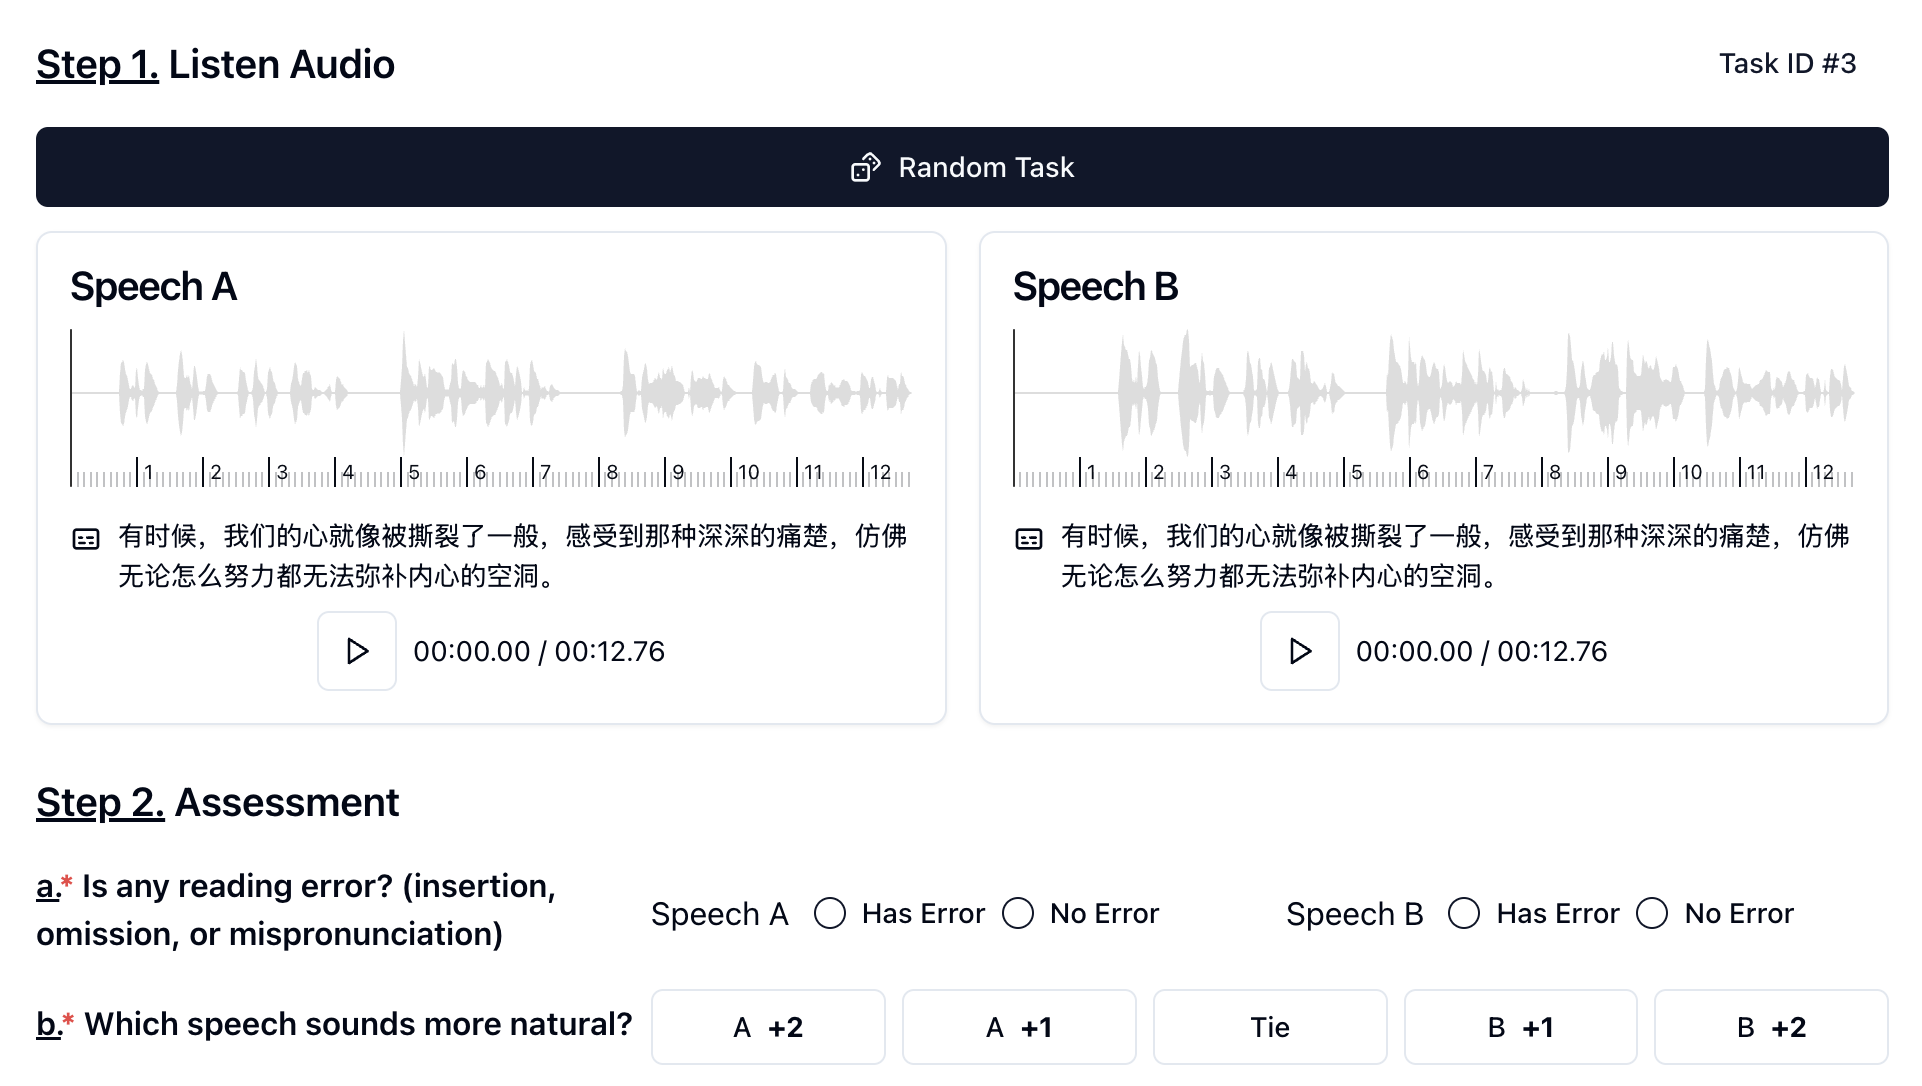
\includegraphics[width=1\linewidth]{img/reading_err_and_natural.png}
    \caption{User interface for intelligibility and naturalness evaluation.}
    \label{fig:reading_err_and_natural}
\end{figure}

\begin{figure}[h]
    \centering
    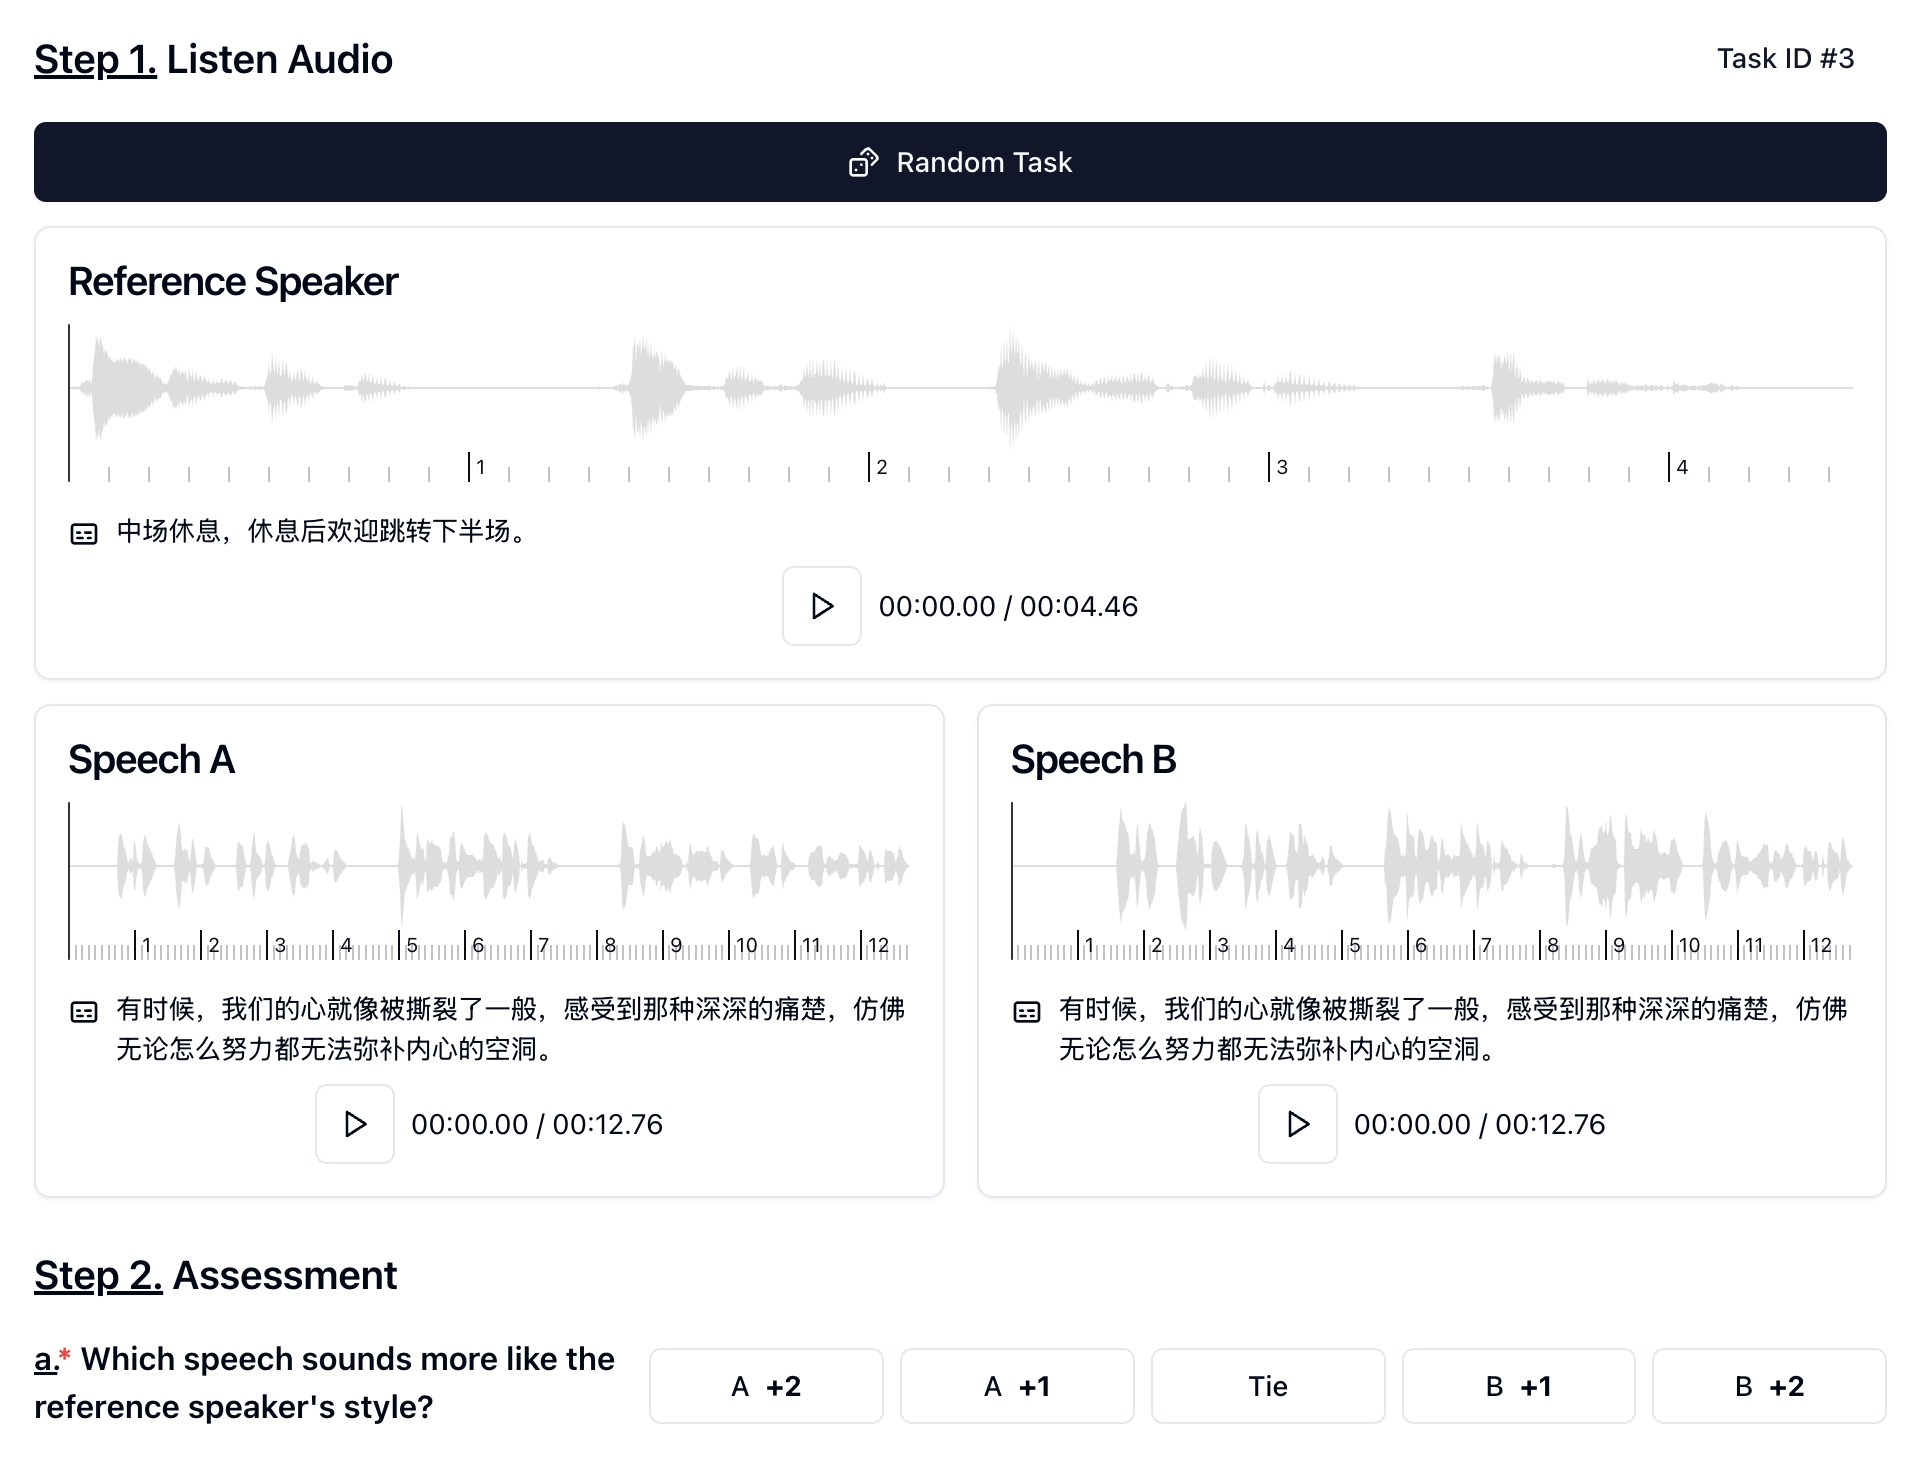
\includegraphics[width=1\linewidth]{img/ref_audio.png}
    \caption{User interface for speaker similarity evaluation.}
    \label{fig:ref_audio}
\end{figure}

We conduct subjective evaluations from three perspectives: intelligibility (reading accuracy), naturalness (N-CMOS), and speaker similarity (A/B Testing). We have developed an automated subjective evaluation interface, as shown in Figure~\ref{fig:reading_err_and_natural} and Figure~\ref{fig:ref_audio}. For each item to be evaluated, users will see three components: the System Interface, the Questionnaire, and the Evaluation Criteria.

    \paragraph{Intelligibility (Reading Accuracy):}
    
    \begin{itemize}[itemsep=0ex,leftmargin=2ex]
        \item \textbf{System Interface:} Users listen to the speech audio and compare it to the provided target text to assess whether the speech matches the text.
        
        \item \textbf{Questionnaire:} Users are asked, ``Is any reading error? (insertion, omission, or mispronunciation)''

         \item \textbf{Evaluation Criteria:} The evaluation is binary: ``No Error'' (the speech matches the text) or ``Has Error'' (the speech does not match the text).
    \end{itemize}
    
    \paragraph{Naturalness (N-CMOS):}
    
    \begin{itemize}[itemsep=0ex,leftmargin=2ex]
        \item \textbf{System Interface:} Users listen to two speech samples, A and B, to compare their naturalness.
        
        \item \textbf{Questionnaire:} Users are asked, ``Which speech sounds more natural?''
        
        \item \textbf{Evaluation Criteria:} Options include A +2 (Sample A is much more natural), A +1 (Sample A is slightly more natural), Tie (Both are equally natural), B +1 (Sample B is slightly more natural), and B +2 (Sample B is much more natural).
    \end{itemize}
    
    \paragraph{Speaker Similarity (A/B Testing):}

    \begin{itemize}[itemsep=0ex,leftmargin=2ex]
        \item \textbf{System Interface:} Users listen to two speech samples, A and B, to evaluate their similarity to the speech of the reference speaker.
        
        \item \textbf{Questionnaire:} Users are asked, ``Which speech sounds more like the reference speaker's style?''
        
        \item \textbf{Evaluation Criteria:} Options include A +2 (Sample A is much more similar), A +1 (Sample A is slightly more similar), Tie (Both are equally similar), B +1 (Sample B is slightly more similar), and B +2 (Sample B is much more similar).
    \end{itemize}


\end{document}
